% **************************************************************************************************************
% A Classic Thesis Style
% An Homage to The Elements of Typographic Style
%
% Copyright (C) 2018 André Miede and Ivo Pletikosić
%
% If you like the style then I would appreciate a postcard. My address
% can be found in the file ClassicThesis.pdf. A collection of the
% postcards I received so far is available online at
% http://postcards.miede.de
%
% License:
% This program is free software; you can redistribute it and/or modify
% it under the terms of the GNU General Public License as published by
% the Free Software Foundation; either version 2 of the License, or
% (at your option) any later version.
%
% This program is distributed in the hope that it will be useful,
% but WITHOUT ANY WARRANTY; without even the implied warranty of
% MERCHANTABILITY or FITNESS FOR A PARTICULAR PURPOSE.  See the
% GNU General Public License for more details.
%
% You should have received a copy of the GNU General Public License
% along with this program; see the file COPYING.  If not, write to
% the Free Software Foundation, Inc., 59 Temple Place - Suite 330,
% Boston, MA 02111-1307, USA.
%
% PLEASE SEE ALSO THE AUTHORS' NOTE REGARDING THIS LICENSE
% IN THE DOCUMENTATION (ClassicThesis.pdf --> Chapter 1 / Chapter01.tex)
% **************************************************************************************************************
\RequirePackage{silence} % :-\
    \WarningFilter{scrreprt}{Usage of package `titlesec'}
    %\WarningFilter{scrreprt}{Activating an ugly workaround}
    \WarningFilter{titlesec}{Non standard sectioning command detected}
\documentclass[ twoside,openright,titlepage,numbers=noenddot,%1headlines,
                headinclude,footinclude,cleardoublepage=empty,abstract=on,
                BCOR=5mm,paper=a4,fontsize=11pt
                ]{scrreprt}

%********************************************************************
% Note: Make all your adjustments in here
%*******************************************************
\usepackage{etoolbox}
\newtoggle{adrianstyle}
%\toggletrue{adrianstyle} % uncomment this line to have smaller margins
\PassOptionsToPackage{adrianstyle=\iftoggle{adrianstyle}{true}{false}}{classicthesis}
\newtoggle{parts}
%\toggletrue{parts} % uncomment to use parts (for long theses only!)
\newtoggle{phd}
%\toggletrue{phd} % uncomment to write a full-blown PhD thesis (with parts, author references, etc.)
\iftoggle{phd}{\toggletrue{parts}}{}

% !TeX root = ./Thesis.tex

% ****************************************************************************************************
% classicthesis-config.tex
% formerly known as loadpackages.sty, classicthesis-ldpkg.sty, and classicthesis-preamble.sty
% Use it at the beginning of your ClassicThesis.tex, or as a LaTeX Preamble
% in your ClassicThesis.{tex,lyx} with % !TeX root = ./Thesis.tex

% ****************************************************************************************************
% classicthesis-config.tex
% formerly known as loadpackages.sty, classicthesis-ldpkg.sty, and classicthesis-preamble.sty
% Use it at the beginning of your ClassicThesis.tex, or as a LaTeX Preamble
% in your ClassicThesis.{tex,lyx} with % !TeX root = ./Thesis.tex

% ****************************************************************************************************
% classicthesis-config.tex
% formerly known as loadpackages.sty, classicthesis-ldpkg.sty, and classicthesis-preamble.sty
% Use it at the beginning of your ClassicThesis.tex, or as a LaTeX Preamble
% in your ClassicThesis.{tex,lyx} with \input{classicthesis-config}
% ****************************************************************************************************
% If you like the classicthesis, then I would appreciate a postcard.
% My address can be found in the file ClassicThesis.pdf. A collection
% of the postcards I received so far is available online at
% http://postcards.miede.de
% ****************************************************************************************************


% ****************************************************************************************************
% 0. Set the encoding of your files. UTF-8 is the only sensible encoding nowadays. If you can't read
% äöüßáéçèê∂åëæƒÏ€ then change the encoding setting in your editor, not the line below. If your editor
% does not support utf8 use another editor!
% ****************************************************************************************************
\PassOptionsToPackage{utf8}{inputenc}
  \usepackage{inputenc}

\PassOptionsToPackage{T1}{fontenc} % T2A for cyrillics
  \usepackage{fontenc}


% ****************************************************************************************************
% 1. Configure classicthesis for your needs here, e.g., remove "drafting" below
% in order to deactivate the time-stamp on the pages
% (see ClassicThesis.pdf for more information):
% ****************************************************************************************************
\PassOptionsToPackage{
  drafting=false,    % print version information on the bottom of the pages
  tocaligned=false, % the left column of the toc will be aligned (no indentation)
  dottedtoc=true,  % page numbers in ToC flushed right
  eulerchapternumbers=true, % use AMS Euler for chapter font (otherwise Palatino)
  linedheaders=false,       % chaper headers will have line above and beneath
  floatperchapter=false,     % numbering per chapter for all floats (i.e., Figure 1.1)
  eulermath=true,  % use awesome Euler fonts for mathematical formulae (only with pdfLaTeX)
  beramono=true,    % toggle a nice monospaced font (w/ bold)
  palatino=true,    % deactivate standard font for loading another one, see the last section at the end of this file for suggestions
  style=classicthesis % classicthesis, arsclassica
}{classicthesis}


% ****************************************************************************************************
% 2. Personal data and user ad-hoc commands (insert your own data here)
% ****************************************************************************************************
\newcommand{\myTitle}{Wirelength Estimation with Neural Networks in VPR}
\newcommand{\myDegree}{Bachelor Thesis}
\newcommand{\myDegreePhD}{Doktor-Ingenieur (Dr.-Ing.)}
\newcommand{\myName}{Vincenz Mechler}
\newcommand{\myNameAndDegree}{\myName, M.\,Sc.} % only for PhD thesis
\newcommand{\myBirthDate}{\formatdate{1}{1}{1970}} % only for PhD thesis
\newcommand{\myBirthPlace}{Darmstadt, Deutschland} % only for PhD thesis
\newcommand{\myNationality}{German} % only for PhD thesis
\newcommand{\myProf}{Prof. Andreas Koch}
\newcommand{\myOtherProf}{Put name here} % only for PhD thesis
\newcommand{\mySupervisor}{Florian Stock}
\newcommand{\myThesiscode}{} % You will get this from our secretary Doris Müller
\newcommand{\myFaculty}{Department of Computer Science}
\newcommand{\myFacultyDE}{Fachbereich Informatik}
\newcommand{\myDepartment}{Embedded Systems and Applications}
\newcommand{\myDepartmentDE}{Eingebettete Systeme und ihre Anwendungen}
\newcommand{\myUni}{\protect{Technische Universität Darmstadt}}
\newcommand{\myUniKennziffer}{D17}
\newcommand{\myLocation}{Darmstadt}
\newcommand{\myTime}{\formatdate{08}{09}{2020}} % hand-in date of the thesis
\newcommand{\myYearPublication}{1337} % year of publication (only for PhD thesis)
\newcommand{\myYearPresent}{1337} % year of disputation (only for PhD thesis)
\newcommand{\myTimePresent}{\formatdate{01}{01}{\myYearPresent}} % date of disputation (only for PhD thesis)
\newcommand{\myVersion}{0.1}
\newcommand{\myURN}{urn:nbn:de:tuda-tuprints-83253} % only for PhD thesis
\newcommand{\myAbstract}{} % at the very end, put your "clean" abstract here

% ********************************************************************
% Setup, finetuning, and useful commands
% ********************************************************************
\providecommand{\mLyX}{L\kern-.1667em\lower.25em\hbox{Y}\kern-.125emX\@}
% ****************************************************************************************************


% ****************************************************************************************************
% 3. Loading some handy packages
% ****************************************************************************************************
% ********************************************************************
% Packages with options that might require adjustments
% ********************************************************************
\PassOptionsToPackage{ngerman,american}{babel} % change this to your language(s), main language last
% Spanish languages need extra options in order to work with this template
%\PassOptionsToPackage{spanish,es-lcroman}{babel}
    \usepackage{babel}

\PassOptionsToPackage{autostyle=true}{csquotes}
    \usepackage{csquotes}
\PassOptionsToPackage{%
  %backend=biber,bibencoding=utf8, %instead of bibtex
  backend=bibtex8,bibencoding=ascii,%
  language=auto,%
  style=numeric-comp,%
  %style=authoryear-comp, % Author 1999, 2010
  %bibstyle=authoryear,dashed=false, % dashed: substitute rep. author with ---
  sorting=nyt, % name, year, title
  maxbibnames=10, % default: 3, et al.
  %backref=true,%
  natbib=true % natbib compatibility mode (\citep and \citet still work)
}{biblatex}
    \usepackage{biblatex}

\PassOptionsToPackage{fleqn}{amsmath}       % math environments and more by the AMS
  \usepackage{amsmath}

% ********************************************************************
% General useful packages
% ********************************************************************
\usepackage{graphicx} %
\usepackage{scrhack} % fix warnings when using KOMA with listings package
\usepackage{xspace} % to get the spacing after macros right
\PassOptionsToPackage{style=long,nopostdot,acronym,shortcuts,nonumberlist,nolist}{glossaries}
  \usepackage{glossaries}
\makeglossary

% ****************************************************************************************************
%\usepackage{pgfplots} % External TikZ/PGF support (thanks to Andreas Nautsch)
%\usetikzlibrary{external}
%\tikzexternalize[mode=list and make, prefix=ext-tikz/]
% ****************************************************************************************************


% ****************************************************************************************************
% 4. Setup floats: tables, (sub)figures, and captions
% ****************************************************************************************************
\usepackage{subcaption}
\usepackage{tabularx} % better tables
  \setlength{\extrarowheight}{3pt} % increase table row height
\newcommand{\tableheadline}[1]{\multicolumn{1}{@{}l@{}}{\spacedlowsmallcaps{#1}}}
\newcommand{\myfloatalign}{\centering} % to be used with each float for alignment
% \usepackage{subfig}
% ****************************************************************************************************


% ****************************************************************************************************
% 5. Setup code listings
% ****************************************************************************************************
\usepackage{listings}
\lstset{
  % color scheme follows template
  commentstyle=\color{CTsemi},
  keywordstyle={\color{CTtitle}},
  stringstyle=\color{CTcitation},
  basicstyle=\ttfamily\lst@ifdisplaystyle\small\fi, % use normal font size in \lstinline
  emphstyle={\color{CTlink}},
  tabsize=2,
  showstringspaces=false,
  captionpos=b, % caption below listing
  %belowcaptionskip=.75\baselineskip
  breaklines=true,
  frame=tb,
  numberstyle=\scriptsize,%\tiny
  numbers=left,%none,%
  stepnumber=1,
  numbersep=8pt,
}
% ****************************************************************************************************




% ****************************************************************************************************
% 6. Last calls before the bar closes
% ****************************************************************************************************
% ********************************************************************
% Her Majesty herself
% ********************************************************************
\usepackage{classicthesis}


% ********************************************************************
% Fine-tune hyperreferences (hyperref should be called last)
% ********************************************************************
\hypersetup{%
  %draft, % hyperref's draft mode, for printing see below
  colorlinks=true, linktocpage=true, pdfstartpage=3, pdfstartview=FitV,%
  % uncomment the following line if you want to have black links (e.g., for printing)
  %colorlinks=false, linktocpage=false, pdfstartpage=3, pdfstartview=FitV, pdfborder={0 0 0},%
  breaklinks=true, pageanchor=true,%
  pdfpagemode=UseNone, %
  % pdfpagemode=UseOutlines,%
  plainpages=false, bookmarksnumbered, bookmarksopen=true, bookmarksopenlevel=1,%
  hypertexnames=true, pdfhighlight=/O,%nesting=true,%frenchlinks,%
  urlcolor=CTurl, linkcolor=CTlink, citecolor=CTcitation, %pagecolor=RoyalBlue,%
  %urlcolor=Black, linkcolor=Black, citecolor=Black, %pagecolor=Black,%
  pdftitle={\myTitle{}},%
  pdfauthor={\textcopyright\ \myName{}, \myUni{}, \myFaculty{}},%
  pdfsubject={\myAbstract},%
  pdfkeywords={},%
  pdfcreator={pdfLaTeX},%
  pdfproducer={LaTeX with hyperref and classicthesis}%
}


% ********************************************************************
% Setup autoreferences (hyperref and babel)
% ********************************************************************
% There are some issues regarding autorefnames
% http://www.tex.ac.uk/cgi-bin/texfaq2html?label=latexwords
% you have to redefine the macros for the
% language you use, e.g., american, ngerman
% (as chosen when loading babel/AtBeginDocument)
% ********************************************************************
\makeatletter
\@ifpackageloaded{babel}%
  {%
    \addto\extrasamerican{%
      \renewcommand*{\figureautorefname}{Figure}%
      \renewcommand*{\tableautorefname}{Table}%
      \renewcommand*{\partautorefname}{Part}%
      \renewcommand*{\chapterautorefname}{Chapter}%
      \renewcommand*{\sectionautorefname}{Section}%
      \renewcommand*{\subsectionautorefname}{Section}%
      \renewcommand*{\subsubsectionautorefname}{Section}%
    }%
    \addto\extrasngerman{%
      \renewcommand*{\paragraphautorefname}{Absatz}%
      \renewcommand*{\subparagraphautorefname}{Unterabsatz}%
      \renewcommand*{\footnoteautorefname}{Fu\"snote}%
      \renewcommand*{\FancyVerbLineautorefname}{Zeile}%
      \renewcommand*{\theoremautorefname}{Theorem}%
      \renewcommand*{\appendixautorefname}{Anhang}%
      \renewcommand*{\equationautorefname}{Gleichung}%
      \renewcommand*{\itemautorefname}{Punkt}%
    }%
      % Fix to getting autorefs for subfigures right (thanks to Belinda Vogt for changing the definition)
      \providecommand{\subfigureautorefname}{\figureautorefname}%
    }{\relax}
\makeatother


% ********************************************************************
% Development Stuff
% ********************************************************************
\listfiles
%\PassOptionsToPackage{l2tabu,orthodox,abort}{nag}
%  \usepackage{nag}
%\PassOptionsToPackage{warning, all}{onlyamsmath}
%  \usepackage{onlyamsmath}


% ****************************************************************************************************
% 7. Further adjustments (experimental)
% ****************************************************************************************************
% ********************************************************************
% Changing the text area
% ********************************************************************
%\areaset[current]{312pt}{761pt} % 686 (factor 2.2) + 33 head + 42 head \the\footskip
%\setlength{\marginparwidth}{7em}%
%\setlength{\marginparsep}{2em}%

% ********************************************************************
% Using different fonts
% ********************************************************************
%\usepackage[oldstylenums]{kpfonts} % oldstyle notextcomp
% \usepackage[osf]{libertine}
%\usepackage[light,condensed,math]{iwona}
%\renewcommand{\sfdefault}{iwona}
%\usepackage{lmodern} % <-- no osf support :-(
%\usepackage{cfr-lm} %
%\usepackage[urw-garamond]{mathdesign} <-- no osf support :-(
%\usepackage[default,osfigures]{opensans} % scale=0.95
%\usepackage[sfdefault]{FiraSans}
% \usepackage[opticals,mathlf]{MinionPro} % onlytext
% ********************************************************************
%\usepackage[largesc,osf]{newpxtext}
%\linespread{1.05} % a bit more for Palatino
% Used to fix these:
% https://bitbucket.org/amiede/classicthesis/issues/139/italics-in-pallatino-capitals-chapter
% https://bitbucket.org/amiede/classicthesis/issues/45/problema-testatine-su-classicthesis-style
% ********************************************************************
% ****************************************************************************************************

% ****************************************************************************************************
% If you like the classicthesis, then I would appreciate a postcard.
% My address can be found in the file ClassicThesis.pdf. A collection
% of the postcards I received so far is available online at
% http://postcards.miede.de
% ****************************************************************************************************


% ****************************************************************************************************
% 0. Set the encoding of your files. UTF-8 is the only sensible encoding nowadays. If you can't read
% äöüßáéçèê∂åëæƒÏ€ then change the encoding setting in your editor, not the line below. If your editor
% does not support utf8 use another editor!
% ****************************************************************************************************
\PassOptionsToPackage{utf8}{inputenc}
  \usepackage{inputenc}

\PassOptionsToPackage{T1}{fontenc} % T2A for cyrillics
  \usepackage{fontenc}


% ****************************************************************************************************
% 1. Configure classicthesis for your needs here, e.g., remove "drafting" below
% in order to deactivate the time-stamp on the pages
% (see ClassicThesis.pdf for more information):
% ****************************************************************************************************
\PassOptionsToPackage{
  drafting=false,    % print version information on the bottom of the pages
  tocaligned=false, % the left column of the toc will be aligned (no indentation)
  dottedtoc=true,  % page numbers in ToC flushed right
  eulerchapternumbers=true, % use AMS Euler for chapter font (otherwise Palatino)
  linedheaders=false,       % chaper headers will have line above and beneath
  floatperchapter=false,     % numbering per chapter for all floats (i.e., Figure 1.1)
  eulermath=true,  % use awesome Euler fonts for mathematical formulae (only with pdfLaTeX)
  beramono=true,    % toggle a nice monospaced font (w/ bold)
  palatino=true,    % deactivate standard font for loading another one, see the last section at the end of this file for suggestions
  style=classicthesis % classicthesis, arsclassica
}{classicthesis}


% ****************************************************************************************************
% 2. Personal data and user ad-hoc commands (insert your own data here)
% ****************************************************************************************************
\newcommand{\myTitle}{Wirelength Estimation with Neural Networks in VPR}
\newcommand{\myDegree}{Bachelor Thesis}
\newcommand{\myDegreePhD}{Doktor-Ingenieur (Dr.-Ing.)}
\newcommand{\myName}{Vincenz Mechler}
\newcommand{\myNameAndDegree}{\myName, M.\,Sc.} % only for PhD thesis
\newcommand{\myBirthDate}{\formatdate{1}{1}{1970}} % only for PhD thesis
\newcommand{\myBirthPlace}{Darmstadt, Deutschland} % only for PhD thesis
\newcommand{\myNationality}{German} % only for PhD thesis
\newcommand{\myProf}{Prof. Andreas Koch}
\newcommand{\myOtherProf}{Put name here} % only for PhD thesis
\newcommand{\mySupervisor}{Florian Stock}
\newcommand{\myThesiscode}{} % You will get this from our secretary Doris Müller
\newcommand{\myFaculty}{Department of Computer Science}
\newcommand{\myFacultyDE}{Fachbereich Informatik}
\newcommand{\myDepartment}{Embedded Systems and Applications}
\newcommand{\myDepartmentDE}{Eingebettete Systeme und ihre Anwendungen}
\newcommand{\myUni}{\protect{Technische Universität Darmstadt}}
\newcommand{\myUniKennziffer}{D17}
\newcommand{\myLocation}{Darmstadt}
\newcommand{\myTime}{\formatdate{08}{09}{2020}} % hand-in date of the thesis
\newcommand{\myYearPublication}{1337} % year of publication (only for PhD thesis)
\newcommand{\myYearPresent}{1337} % year of disputation (only for PhD thesis)
\newcommand{\myTimePresent}{\formatdate{01}{01}{\myYearPresent}} % date of disputation (only for PhD thesis)
\newcommand{\myVersion}{0.1}
\newcommand{\myURN}{urn:nbn:de:tuda-tuprints-83253} % only for PhD thesis
\newcommand{\myAbstract}{} % at the very end, put your "clean" abstract here

% ********************************************************************
% Setup, finetuning, and useful commands
% ********************************************************************
\providecommand{\mLyX}{L\kern-.1667em\lower.25em\hbox{Y}\kern-.125emX\@}
% ****************************************************************************************************


% ****************************************************************************************************
% 3. Loading some handy packages
% ****************************************************************************************************
% ********************************************************************
% Packages with options that might require adjustments
% ********************************************************************
\PassOptionsToPackage{ngerman,american}{babel} % change this to your language(s), main language last
% Spanish languages need extra options in order to work with this template
%\PassOptionsToPackage{spanish,es-lcroman}{babel}
    \usepackage{babel}

\PassOptionsToPackage{autostyle=true}{csquotes}
    \usepackage{csquotes}
\PassOptionsToPackage{%
  %backend=biber,bibencoding=utf8, %instead of bibtex
  backend=bibtex8,bibencoding=ascii,%
  language=auto,%
  style=numeric-comp,%
  %style=authoryear-comp, % Author 1999, 2010
  %bibstyle=authoryear,dashed=false, % dashed: substitute rep. author with ---
  sorting=nyt, % name, year, title
  maxbibnames=10, % default: 3, et al.
  %backref=true,%
  natbib=true % natbib compatibility mode (\citep and \citet still work)
}{biblatex}
    \usepackage{biblatex}

\PassOptionsToPackage{fleqn}{amsmath}       % math environments and more by the AMS
  \usepackage{amsmath}

% ********************************************************************
% General useful packages
% ********************************************************************
\usepackage{graphicx} %
\usepackage{scrhack} % fix warnings when using KOMA with listings package
\usepackage{xspace} % to get the spacing after macros right
\PassOptionsToPackage{style=long,nopostdot,acronym,shortcuts,nonumberlist,nolist}{glossaries}
  \usepackage{glossaries}
\makeglossary

% ****************************************************************************************************
%\usepackage{pgfplots} % External TikZ/PGF support (thanks to Andreas Nautsch)
%\usetikzlibrary{external}
%\tikzexternalize[mode=list and make, prefix=ext-tikz/]
% ****************************************************************************************************


% ****************************************************************************************************
% 4. Setup floats: tables, (sub)figures, and captions
% ****************************************************************************************************
\usepackage{subcaption}
\usepackage{tabularx} % better tables
  \setlength{\extrarowheight}{3pt} % increase table row height
\newcommand{\tableheadline}[1]{\multicolumn{1}{@{}l@{}}{\spacedlowsmallcaps{#1}}}
\newcommand{\myfloatalign}{\centering} % to be used with each float for alignment
% \usepackage{subfig}
% ****************************************************************************************************


% ****************************************************************************************************
% 5. Setup code listings
% ****************************************************************************************************
\usepackage{listings}
\lstset{
  % color scheme follows template
  commentstyle=\color{CTsemi},
  keywordstyle={\color{CTtitle}},
  stringstyle=\color{CTcitation},
  basicstyle=\ttfamily\lst@ifdisplaystyle\small\fi, % use normal font size in \lstinline
  emphstyle={\color{CTlink}},
  tabsize=2,
  showstringspaces=false,
  captionpos=b, % caption below listing
  %belowcaptionskip=.75\baselineskip
  breaklines=true,
  frame=tb,
  numberstyle=\scriptsize,%\tiny
  numbers=left,%none,%
  stepnumber=1,
  numbersep=8pt,
}
% ****************************************************************************************************




% ****************************************************************************************************
% 6. Last calls before the bar closes
% ****************************************************************************************************
% ********************************************************************
% Her Majesty herself
% ********************************************************************
\usepackage{classicthesis}


% ********************************************************************
% Fine-tune hyperreferences (hyperref should be called last)
% ********************************************************************
\hypersetup{%
  %draft, % hyperref's draft mode, for printing see below
  colorlinks=true, linktocpage=true, pdfstartpage=3, pdfstartview=FitV,%
  % uncomment the following line if you want to have black links (e.g., for printing)
  %colorlinks=false, linktocpage=false, pdfstartpage=3, pdfstartview=FitV, pdfborder={0 0 0},%
  breaklinks=true, pageanchor=true,%
  pdfpagemode=UseNone, %
  % pdfpagemode=UseOutlines,%
  plainpages=false, bookmarksnumbered, bookmarksopen=true, bookmarksopenlevel=1,%
  hypertexnames=true, pdfhighlight=/O,%nesting=true,%frenchlinks,%
  urlcolor=CTurl, linkcolor=CTlink, citecolor=CTcitation, %pagecolor=RoyalBlue,%
  %urlcolor=Black, linkcolor=Black, citecolor=Black, %pagecolor=Black,%
  pdftitle={\myTitle{}},%
  pdfauthor={\textcopyright\ \myName{}, \myUni{}, \myFaculty{}},%
  pdfsubject={\myAbstract},%
  pdfkeywords={},%
  pdfcreator={pdfLaTeX},%
  pdfproducer={LaTeX with hyperref and classicthesis}%
}


% ********************************************************************
% Setup autoreferences (hyperref and babel)
% ********************************************************************
% There are some issues regarding autorefnames
% http://www.tex.ac.uk/cgi-bin/texfaq2html?label=latexwords
% you have to redefine the macros for the
% language you use, e.g., american, ngerman
% (as chosen when loading babel/AtBeginDocument)
% ********************************************************************
\makeatletter
\@ifpackageloaded{babel}%
  {%
    \addto\extrasamerican{%
      \renewcommand*{\figureautorefname}{Figure}%
      \renewcommand*{\tableautorefname}{Table}%
      \renewcommand*{\partautorefname}{Part}%
      \renewcommand*{\chapterautorefname}{Chapter}%
      \renewcommand*{\sectionautorefname}{Section}%
      \renewcommand*{\subsectionautorefname}{Section}%
      \renewcommand*{\subsubsectionautorefname}{Section}%
    }%
    \addto\extrasngerman{%
      \renewcommand*{\paragraphautorefname}{Absatz}%
      \renewcommand*{\subparagraphautorefname}{Unterabsatz}%
      \renewcommand*{\footnoteautorefname}{Fu\"snote}%
      \renewcommand*{\FancyVerbLineautorefname}{Zeile}%
      \renewcommand*{\theoremautorefname}{Theorem}%
      \renewcommand*{\appendixautorefname}{Anhang}%
      \renewcommand*{\equationautorefname}{Gleichung}%
      \renewcommand*{\itemautorefname}{Punkt}%
    }%
      % Fix to getting autorefs for subfigures right (thanks to Belinda Vogt for changing the definition)
      \providecommand{\subfigureautorefname}{\figureautorefname}%
    }{\relax}
\makeatother


% ********************************************************************
% Development Stuff
% ********************************************************************
\listfiles
%\PassOptionsToPackage{l2tabu,orthodox,abort}{nag}
%  \usepackage{nag}
%\PassOptionsToPackage{warning, all}{onlyamsmath}
%  \usepackage{onlyamsmath}


% ****************************************************************************************************
% 7. Further adjustments (experimental)
% ****************************************************************************************************
% ********************************************************************
% Changing the text area
% ********************************************************************
%\areaset[current]{312pt}{761pt} % 686 (factor 2.2) + 33 head + 42 head \the\footskip
%\setlength{\marginparwidth}{7em}%
%\setlength{\marginparsep}{2em}%

% ********************************************************************
% Using different fonts
% ********************************************************************
%\usepackage[oldstylenums]{kpfonts} % oldstyle notextcomp
% \usepackage[osf]{libertine}
%\usepackage[light,condensed,math]{iwona}
%\renewcommand{\sfdefault}{iwona}
%\usepackage{lmodern} % <-- no osf support :-(
%\usepackage{cfr-lm} %
%\usepackage[urw-garamond]{mathdesign} <-- no osf support :-(
%\usepackage[default,osfigures]{opensans} % scale=0.95
%\usepackage[sfdefault]{FiraSans}
% \usepackage[opticals,mathlf]{MinionPro} % onlytext
% ********************************************************************
%\usepackage[largesc,osf]{newpxtext}
%\linespread{1.05} % a bit more for Palatino
% Used to fix these:
% https://bitbucket.org/amiede/classicthesis/issues/139/italics-in-pallatino-capitals-chapter
% https://bitbucket.org/amiede/classicthesis/issues/45/problema-testatine-su-classicthesis-style
% ********************************************************************
% ****************************************************************************************************

% ****************************************************************************************************
% If you like the classicthesis, then I would appreciate a postcard.
% My address can be found in the file ClassicThesis.pdf. A collection
% of the postcards I received so far is available online at
% http://postcards.miede.de
% ****************************************************************************************************


% ****************************************************************************************************
% 0. Set the encoding of your files. UTF-8 is the only sensible encoding nowadays. If you can't read
% äöüßáéçèê∂åëæƒÏ€ then change the encoding setting in your editor, not the line below. If your editor
% does not support utf8 use another editor!
% ****************************************************************************************************
\PassOptionsToPackage{utf8}{inputenc}
  \usepackage{inputenc}

\PassOptionsToPackage{T1}{fontenc} % T2A for cyrillics
  \usepackage{fontenc}


% ****************************************************************************************************
% 1. Configure classicthesis for your needs here, e.g., remove "drafting" below
% in order to deactivate the time-stamp on the pages
% (see ClassicThesis.pdf for more information):
% ****************************************************************************************************
\PassOptionsToPackage{
  drafting=false,    % print version information on the bottom of the pages
  tocaligned=false, % the left column of the toc will be aligned (no indentation)
  dottedtoc=true,  % page numbers in ToC flushed right
  eulerchapternumbers=true, % use AMS Euler for chapter font (otherwise Palatino)
  linedheaders=false,       % chaper headers will have line above and beneath
  floatperchapter=false,     % numbering per chapter for all floats (i.e., Figure 1.1)
  eulermath=true,  % use awesome Euler fonts for mathematical formulae (only with pdfLaTeX)
  beramono=true,    % toggle a nice monospaced font (w/ bold)
  palatino=true,    % deactivate standard font for loading another one, see the last section at the end of this file for suggestions
  style=classicthesis % classicthesis, arsclassica
}{classicthesis}


% ****************************************************************************************************
% 2. Personal data and user ad-hoc commands (insert your own data here)
% ****************************************************************************************************
\newcommand{\myTitle}{Wirelength Estimation with Neural Networks in VPR}
\newcommand{\myDegree}{Bachelor Thesis}
\newcommand{\myDegreePhD}{Doktor-Ingenieur (Dr.-Ing.)}
\newcommand{\myName}{Vincenz Mechler}
\newcommand{\myNameAndDegree}{\myName, M.\,Sc.} % only for PhD thesis
\newcommand{\myBirthDate}{\formatdate{1}{1}{1970}} % only for PhD thesis
\newcommand{\myBirthPlace}{Darmstadt, Deutschland} % only for PhD thesis
\newcommand{\myNationality}{German} % only for PhD thesis
\newcommand{\myProf}{Prof. Andreas Koch}
\newcommand{\myOtherProf}{Put name here} % only for PhD thesis
\newcommand{\mySupervisor}{Florian Stock}
\newcommand{\myThesiscode}{} % You will get this from our secretary Doris Müller
\newcommand{\myFaculty}{Department of Computer Science}
\newcommand{\myFacultyDE}{Fachbereich Informatik}
\newcommand{\myDepartment}{Embedded Systems and Applications}
\newcommand{\myDepartmentDE}{Eingebettete Systeme und ihre Anwendungen}
\newcommand{\myUni}{\protect{Technische Universität Darmstadt}}
\newcommand{\myUniKennziffer}{D17}
\newcommand{\myLocation}{Darmstadt}
\newcommand{\myTime}{\formatdate{08}{09}{2020}} % hand-in date of the thesis
\newcommand{\myYearPublication}{1337} % year of publication (only for PhD thesis)
\newcommand{\myYearPresent}{1337} % year of disputation (only for PhD thesis)
\newcommand{\myTimePresent}{\formatdate{01}{01}{\myYearPresent}} % date of disputation (only for PhD thesis)
\newcommand{\myVersion}{0.1}
\newcommand{\myURN}{urn:nbn:de:tuda-tuprints-83253} % only for PhD thesis
\newcommand{\myAbstract}{} % at the very end, put your "clean" abstract here

% ********************************************************************
% Setup, finetuning, and useful commands
% ********************************************************************
\providecommand{\mLyX}{L\kern-.1667em\lower.25em\hbox{Y}\kern-.125emX\@}
% ****************************************************************************************************


% ****************************************************************************************************
% 3. Loading some handy packages
% ****************************************************************************************************
% ********************************************************************
% Packages with options that might require adjustments
% ********************************************************************
\PassOptionsToPackage{ngerman,american}{babel} % change this to your language(s), main language last
% Spanish languages need extra options in order to work with this template
%\PassOptionsToPackage{spanish,es-lcroman}{babel}
    \usepackage{babel}

\PassOptionsToPackage{autostyle=true}{csquotes}
    \usepackage{csquotes}
\PassOptionsToPackage{%
  %backend=biber,bibencoding=utf8, %instead of bibtex
  backend=bibtex8,bibencoding=ascii,%
  language=auto,%
  style=numeric-comp,%
  %style=authoryear-comp, % Author 1999, 2010
  %bibstyle=authoryear,dashed=false, % dashed: substitute rep. author with ---
  sorting=nyt, % name, year, title
  maxbibnames=10, % default: 3, et al.
  %backref=true,%
  natbib=true % natbib compatibility mode (\citep and \citet still work)
}{biblatex}
    \usepackage{biblatex}

\PassOptionsToPackage{fleqn}{amsmath}       % math environments and more by the AMS
  \usepackage{amsmath}

% ********************************************************************
% General useful packages
% ********************************************************************
\usepackage{graphicx} %
\usepackage{scrhack} % fix warnings when using KOMA with listings package
\usepackage{xspace} % to get the spacing after macros right
\PassOptionsToPackage{style=long,nopostdot,acronym,shortcuts,nonumberlist,nolist}{glossaries}
  \usepackage{glossaries}
\makeglossary

% ****************************************************************************************************
%\usepackage{pgfplots} % External TikZ/PGF support (thanks to Andreas Nautsch)
%\usetikzlibrary{external}
%\tikzexternalize[mode=list and make, prefix=ext-tikz/]
% ****************************************************************************************************


% ****************************************************************************************************
% 4. Setup floats: tables, (sub)figures, and captions
% ****************************************************************************************************
\usepackage{subcaption}
\usepackage{tabularx} % better tables
  \setlength{\extrarowheight}{3pt} % increase table row height
\newcommand{\tableheadline}[1]{\multicolumn{1}{@{}l@{}}{\spacedlowsmallcaps{#1}}}
\newcommand{\myfloatalign}{\centering} % to be used with each float for alignment
% \usepackage{subfig}
% ****************************************************************************************************


% ****************************************************************************************************
% 5. Setup code listings
% ****************************************************************************************************
\usepackage{listings}
\lstset{
  % color scheme follows template
  commentstyle=\color{CTsemi},
  keywordstyle={\color{CTtitle}},
  stringstyle=\color{CTcitation},
  basicstyle=\ttfamily\lst@ifdisplaystyle\small\fi, % use normal font size in \lstinline
  emphstyle={\color{CTlink}},
  tabsize=2,
  showstringspaces=false,
  captionpos=b, % caption below listing
  %belowcaptionskip=.75\baselineskip
  breaklines=true,
  frame=tb,
  numberstyle=\scriptsize,%\tiny
  numbers=left,%none,%
  stepnumber=1,
  numbersep=8pt,
}
% ****************************************************************************************************




% ****************************************************************************************************
% 6. Last calls before the bar closes
% ****************************************************************************************************
% ********************************************************************
% Her Majesty herself
% ********************************************************************
\usepackage{classicthesis}


% ********************************************************************
% Fine-tune hyperreferences (hyperref should be called last)
% ********************************************************************
\hypersetup{%
  %draft, % hyperref's draft mode, for printing see below
  colorlinks=true, linktocpage=true, pdfstartpage=3, pdfstartview=FitV,%
  % uncomment the following line if you want to have black links (e.g., for printing)
  %colorlinks=false, linktocpage=false, pdfstartpage=3, pdfstartview=FitV, pdfborder={0 0 0},%
  breaklinks=true, pageanchor=true,%
  pdfpagemode=UseNone, %
  % pdfpagemode=UseOutlines,%
  plainpages=false, bookmarksnumbered, bookmarksopen=true, bookmarksopenlevel=1,%
  hypertexnames=true, pdfhighlight=/O,%nesting=true,%frenchlinks,%
  urlcolor=CTurl, linkcolor=CTlink, citecolor=CTcitation, %pagecolor=RoyalBlue,%
  %urlcolor=Black, linkcolor=Black, citecolor=Black, %pagecolor=Black,%
  pdftitle={\myTitle{}},%
  pdfauthor={\textcopyright\ \myName{}, \myUni{}, \myFaculty{}},%
  pdfsubject={\myAbstract},%
  pdfkeywords={},%
  pdfcreator={pdfLaTeX},%
  pdfproducer={LaTeX with hyperref and classicthesis}%
}


% ********************************************************************
% Setup autoreferences (hyperref and babel)
% ********************************************************************
% There are some issues regarding autorefnames
% http://www.tex.ac.uk/cgi-bin/texfaq2html?label=latexwords
% you have to redefine the macros for the
% language you use, e.g., american, ngerman
% (as chosen when loading babel/AtBeginDocument)
% ********************************************************************
\makeatletter
\@ifpackageloaded{babel}%
  {%
    \addto\extrasamerican{%
      \renewcommand*{\figureautorefname}{Figure}%
      \renewcommand*{\tableautorefname}{Table}%
      \renewcommand*{\partautorefname}{Part}%
      \renewcommand*{\chapterautorefname}{Chapter}%
      \renewcommand*{\sectionautorefname}{Section}%
      \renewcommand*{\subsectionautorefname}{Section}%
      \renewcommand*{\subsubsectionautorefname}{Section}%
    }%
    \addto\extrasngerman{%
      \renewcommand*{\paragraphautorefname}{Absatz}%
      \renewcommand*{\subparagraphautorefname}{Unterabsatz}%
      \renewcommand*{\footnoteautorefname}{Fu\"snote}%
      \renewcommand*{\FancyVerbLineautorefname}{Zeile}%
      \renewcommand*{\theoremautorefname}{Theorem}%
      \renewcommand*{\appendixautorefname}{Anhang}%
      \renewcommand*{\equationautorefname}{Gleichung}%
      \renewcommand*{\itemautorefname}{Punkt}%
    }%
      % Fix to getting autorefs for subfigures right (thanks to Belinda Vogt for changing the definition)
      \providecommand{\subfigureautorefname}{\figureautorefname}%
    }{\relax}
\makeatother


% ********************************************************************
% Development Stuff
% ********************************************************************
\listfiles
%\PassOptionsToPackage{l2tabu,orthodox,abort}{nag}
%  \usepackage{nag}
%\PassOptionsToPackage{warning, all}{onlyamsmath}
%  \usepackage{onlyamsmath}


% ****************************************************************************************************
% 7. Further adjustments (experimental)
% ****************************************************************************************************
% ********************************************************************
% Changing the text area
% ********************************************************************
%\areaset[current]{312pt}{761pt} % 686 (factor 2.2) + 33 head + 42 head \the\footskip
%\setlength{\marginparwidth}{7em}%
%\setlength{\marginparsep}{2em}%

% ********************************************************************
% Using different fonts
% ********************************************************************
%\usepackage[oldstylenums]{kpfonts} % oldstyle notextcomp
% \usepackage[osf]{libertine}
%\usepackage[light,condensed,math]{iwona}
%\renewcommand{\sfdefault}{iwona}
%\usepackage{lmodern} % <-- no osf support :-(
%\usepackage{cfr-lm} %
%\usepackage[urw-garamond]{mathdesign} <-- no osf support :-(
%\usepackage[default,osfigures]{opensans} % scale=0.95
%\usepackage[sfdefault]{FiraSans}
% \usepackage[opticals,mathlf]{MinionPro} % onlytext
% ********************************************************************
%\usepackage[largesc,osf]{newpxtext}
%\linespread{1.05} % a bit more for Palatino
% Used to fix these:
% https://bitbucket.org/amiede/classicthesis/issues/139/italics-in-pallatino-capitals-chapter
% https://bitbucket.org/amiede/classicthesis/issues/45/problema-testatine-su-classicthesis-style
% ********************************************************************
% ****************************************************************************************************

% !TeX root = ./Thesis.tex

\PassOptionsToPackage{capitalize,noabbrev,ngerman,english}{cleveref} % need to pass languages explicitly
	\usepackage{cleveref}

\usepackage{datetime} % for formating submission date

\usepackage{lipsum} % for template text

\usepackage{float}

\iftoggle{phd}{
	\usepackage[LabelsAligned]{currvita} % nice cv style
}{}

\newcommand{\shorturl}[2]{\href{#1}{\nolinkurl{#2}}} % useful for typesetting DOIs and URNs

% TikZ/PGFPlots
\usepackage{tikz}
\usepackage{pgfplots}
\pgfplotsset{compat=newest}
\usetikzlibrary{dsp,chains}
\usetikzlibrary{positioning}
%\DeclareMathAlphabet{\mathpzc}{OT1}{pzc}{m}{it}
%\newcommand{\z}{\mathpzc{z}}
% To cache tikz pictures you have to run pdflatex with -shell-escape or --enable-write18
\ifnum\pdfshellescape=1
\usepgfplotslibrary{external}
\tikzexternalize[prefix=gfxcompiled/]
\fi

% Lengths for matlab2tikz
\newlength\figureheight
\newlength\figurewidth 


%********************************************************************
% Bibliographies
%*******************************************************
\addbibresource{Bibliography.bib}
\addbibresource[label=ownpubs]{AuthorPublications.bib}

%********************************************************************
% Hyphenation
%*******************************************************
% !TeX root = ./Thesis.tex

\hyphenation{
Si-mu-link
OO-WARP-Lab
WARP-Lab
}


%********************************************************************
% Acronyms
%*******************************************************
% !TeX root = ./Thesis.tex
\newacronym{FPGA}{FPGA}{field-programmable gate array}

\newacronym{VPR}{VPR}{Versatile Place and Route}
\newacronym{HPWL}{HPWL}{Half Perimeter Wire Length}
\newacronym{NN}{NN}{Neural Network}
\newacronym{CNN}{CNN}{Convolutional Neural Network}
\newacronym{RNN}{RNN}{Recurrent Neural Network}
\newacronym{tf}{TF}{TensorFlow}
\newacronym{BB}{BB}{bounding box}
\newacronym{HPO}{HPO}{Hyperparameter Optimization}


%********************************************************************
% Macros
%*******************************************************
% !TeX root = ./Thesis.tex

\newcommand{\ie}{i.\,e.}
\newcommand{\Ie}{I.\,e.}
\newcommand{\eg}{e.\,g.}
\newcommand{\Eg}{E.\,g.}
% for use in unnumbered chapters in the front and back matter that should appear in ToC
\newcommand{\chapterExtra}[1]{
	\phantomsection
	\markboth{\spacedlowsmallcaps{#1}}{\spacedlowsmallcaps{#1}}%
	\addcontentsline{toc}{chapter}{\tocEntry{#1}}%
	\chapter*{#1}%
}


% ****************************************************************************************************
% PDF/A for TUbama
% ****************************************************************************************************
\usepackage[binary-units]{siunitx}
\usepackage[a-1b]{pdfx}
\usepackage{filecontents}
\begin{filecontents*}{\jobname.xmpdata}
\Title{\myTitle}
\Author{\myName}
\Copyright{Copyright \copyright\ \myYearPublication "\myName"}
\Keywords{} % \Keywords{Wi-Fi\sep Reverse Engineering\sep macOS}
\Subject{\myAbstract}
\end{filecontents*}

% ********************************************************************
% GO!GO!GO! MOVE IT!
%*******************************************************
\begin{document}
\frenchspacing
\raggedbottom
\selectlanguage{american} % american ngerman
%\renewcommand*{\bibname}{new name}
%\setbibpreamble{}
\pagenumbering{roman}
\pagestyle{plain}
%********************************************************************
% Frontmatter
%*******************************************************
\iftoggle{phd}{
	% !TeX root = ../Thesis.tex

% Vorgaben zum Titelblatt einer Dissertation: https://www.intern.tu-darmstadt.de/media/dezernat_ii/promotionen_dokumente/Dissertation-Titelblatt.de.pdf

%*******************************************************
% Titlepage
%*******************************************************
\pdfbookmark[1]{Cover}{cover}
\begin{titlepage}
    %\pdfbookmark[1]{\myTitle{}}{titlepage}
    % if you want the titlepage to be centered, uncomment and fine-tune the line below (KOMA classes environment)
    \begin{addmargin}[-1cm]{\iftoggle{adrianstyle}{-2cm}{-3cm}}
    \begin{center}
    \begin{otherlanguage}{ngerman}
        \large

        
\includegraphics[width=6cm]{gfx/logos/tud_logo}
        
        \vfill

        \begingroup
            \color{CTtitle}\spacedallcaps{\myTitle{}} \\ \bigskip
        \endgroup

        \vfill

        Vom \myFacultyDE{} der \\ 
        \myUni{} genehmigte

        \vspace{2ex}

        \spacedlowsmallcaps{Dissertation}

        \vspace{2ex}

        zur Erlangung des akademischen Grades \\
        \myDegreePhD{}
        
        \vspace{2ex}

        von

        \vspace{2ex}

        \spacedlowsmallcaps{\myNameAndDegree{}}

        \vspace{2ex}
        
        geboren am \myBirthDate{} in \myBirthPlace{}.

        \vfill

        \begin{tabular}{r@{~}l}
        Erstreferent: & \myProf{} \\
        Korreferent: & \myOtherProf{} \\
        \end{tabular}

        \vfill
        
        \myLocation{} \myYearPresent{} \\
        Hochschulkennziffer \myUniKennziffer{}

        \vfill

        
\includegraphics[width=5cm]{gfx/logos/seemoo_logo} \\

    \end{otherlanguage}
    \end{center}
    \end{addmargin}
\end{titlepage}

	% !TeX root = ../Thesis.tex

% Vorgaben zum Titelblatt einer Dissertation: https://www.intern.tu-darmstadt.de/media/dezernat_ii/promotionen_dokumente/Dissertation-Titelblatt.de.pdf

\thispagestyle{empty}

\ \vfill

\noindent%
\myName{}, \emph{\myTitle{}}, Dissertation, \myUni{}, \myYearPublication{}.

\bigskip

\begin{otherlanguage}{ngerman}

\noindent%
\myDepartmentDE{} \\
\myFacultyDE{} \\
\myUni{} \\
Jahr der Veröffentlichung: \myYearPublication{} \\
Tag der mündlichen Prüfung: \myTimePresent{} \\
URN: \shorturl{https://nbn-resolving.org/\myURN}{\myURN} \\

\bigskip

\noindent%
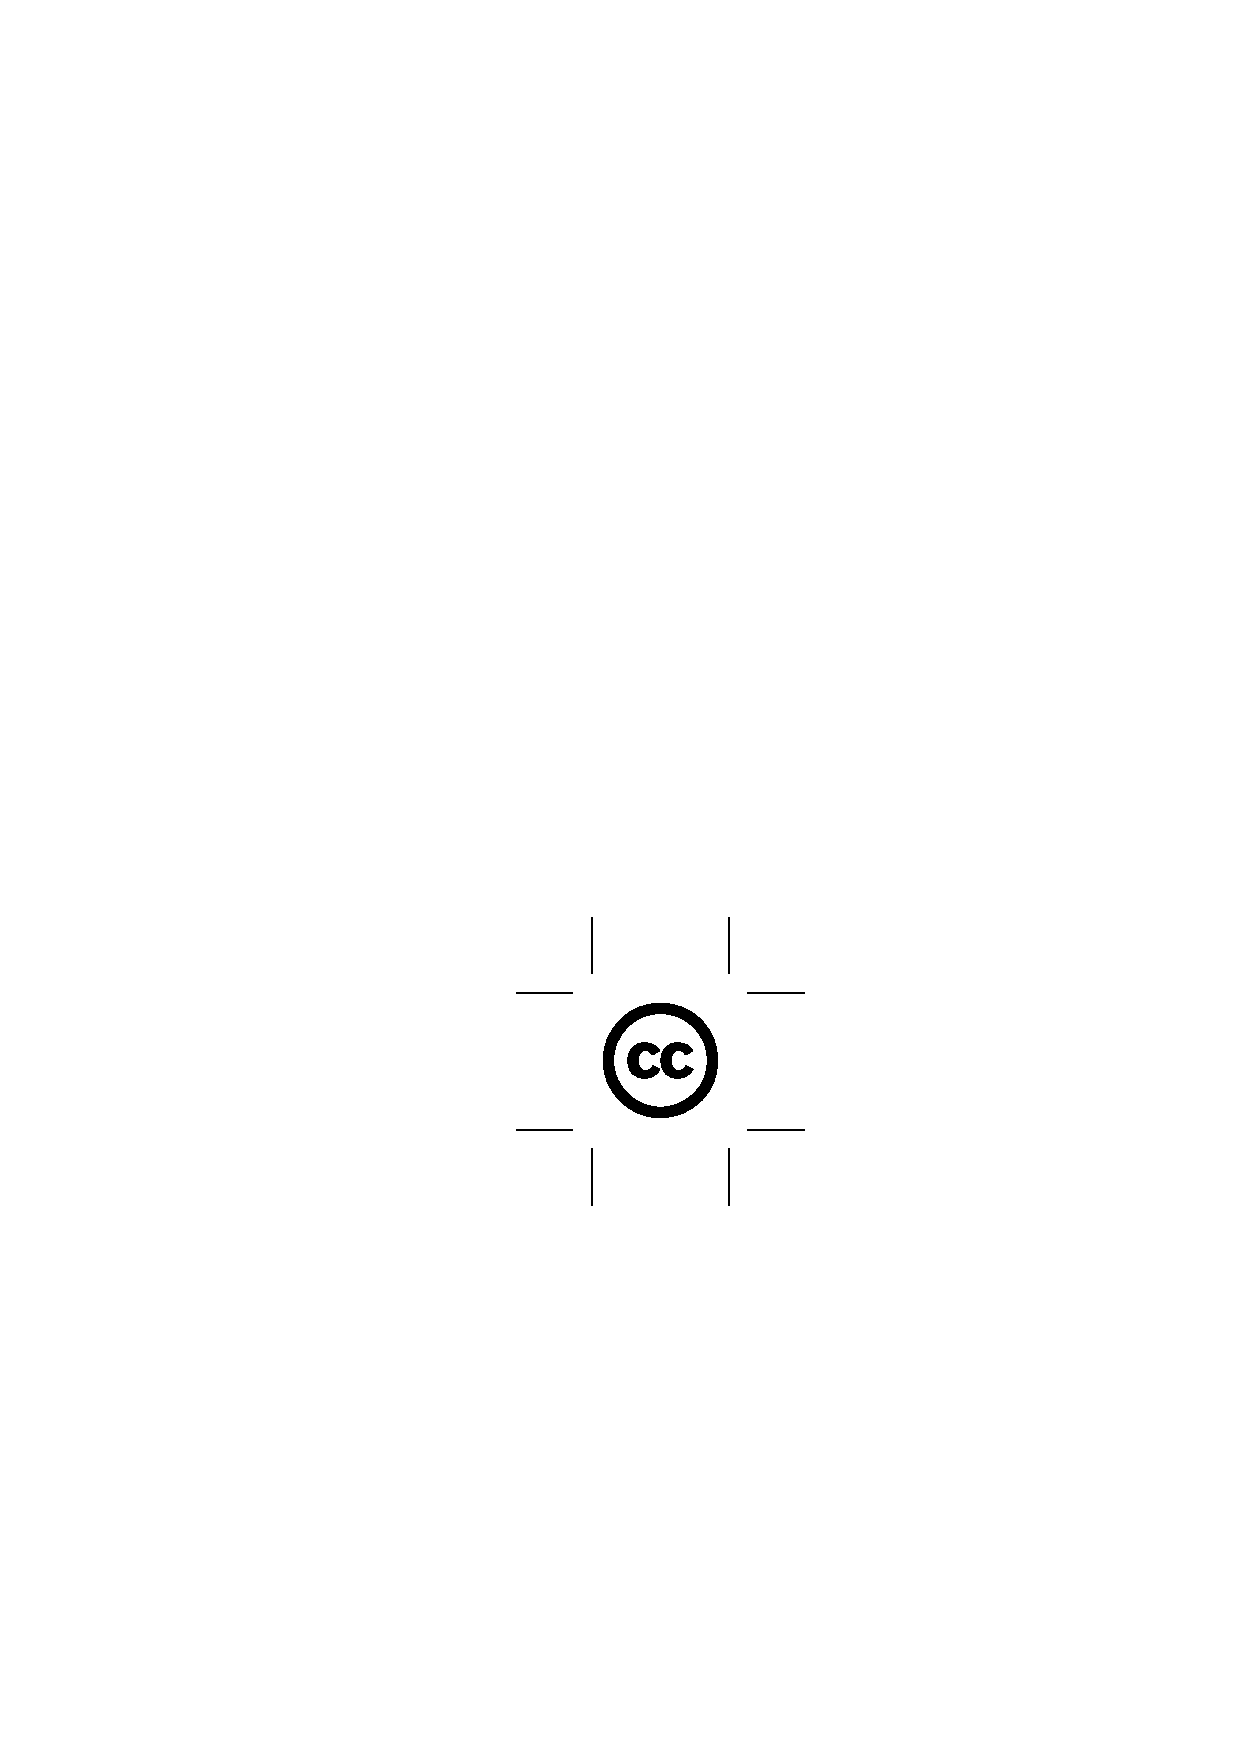
\includegraphics[height=4ex]{gfx/logos/creativecommons/cc}
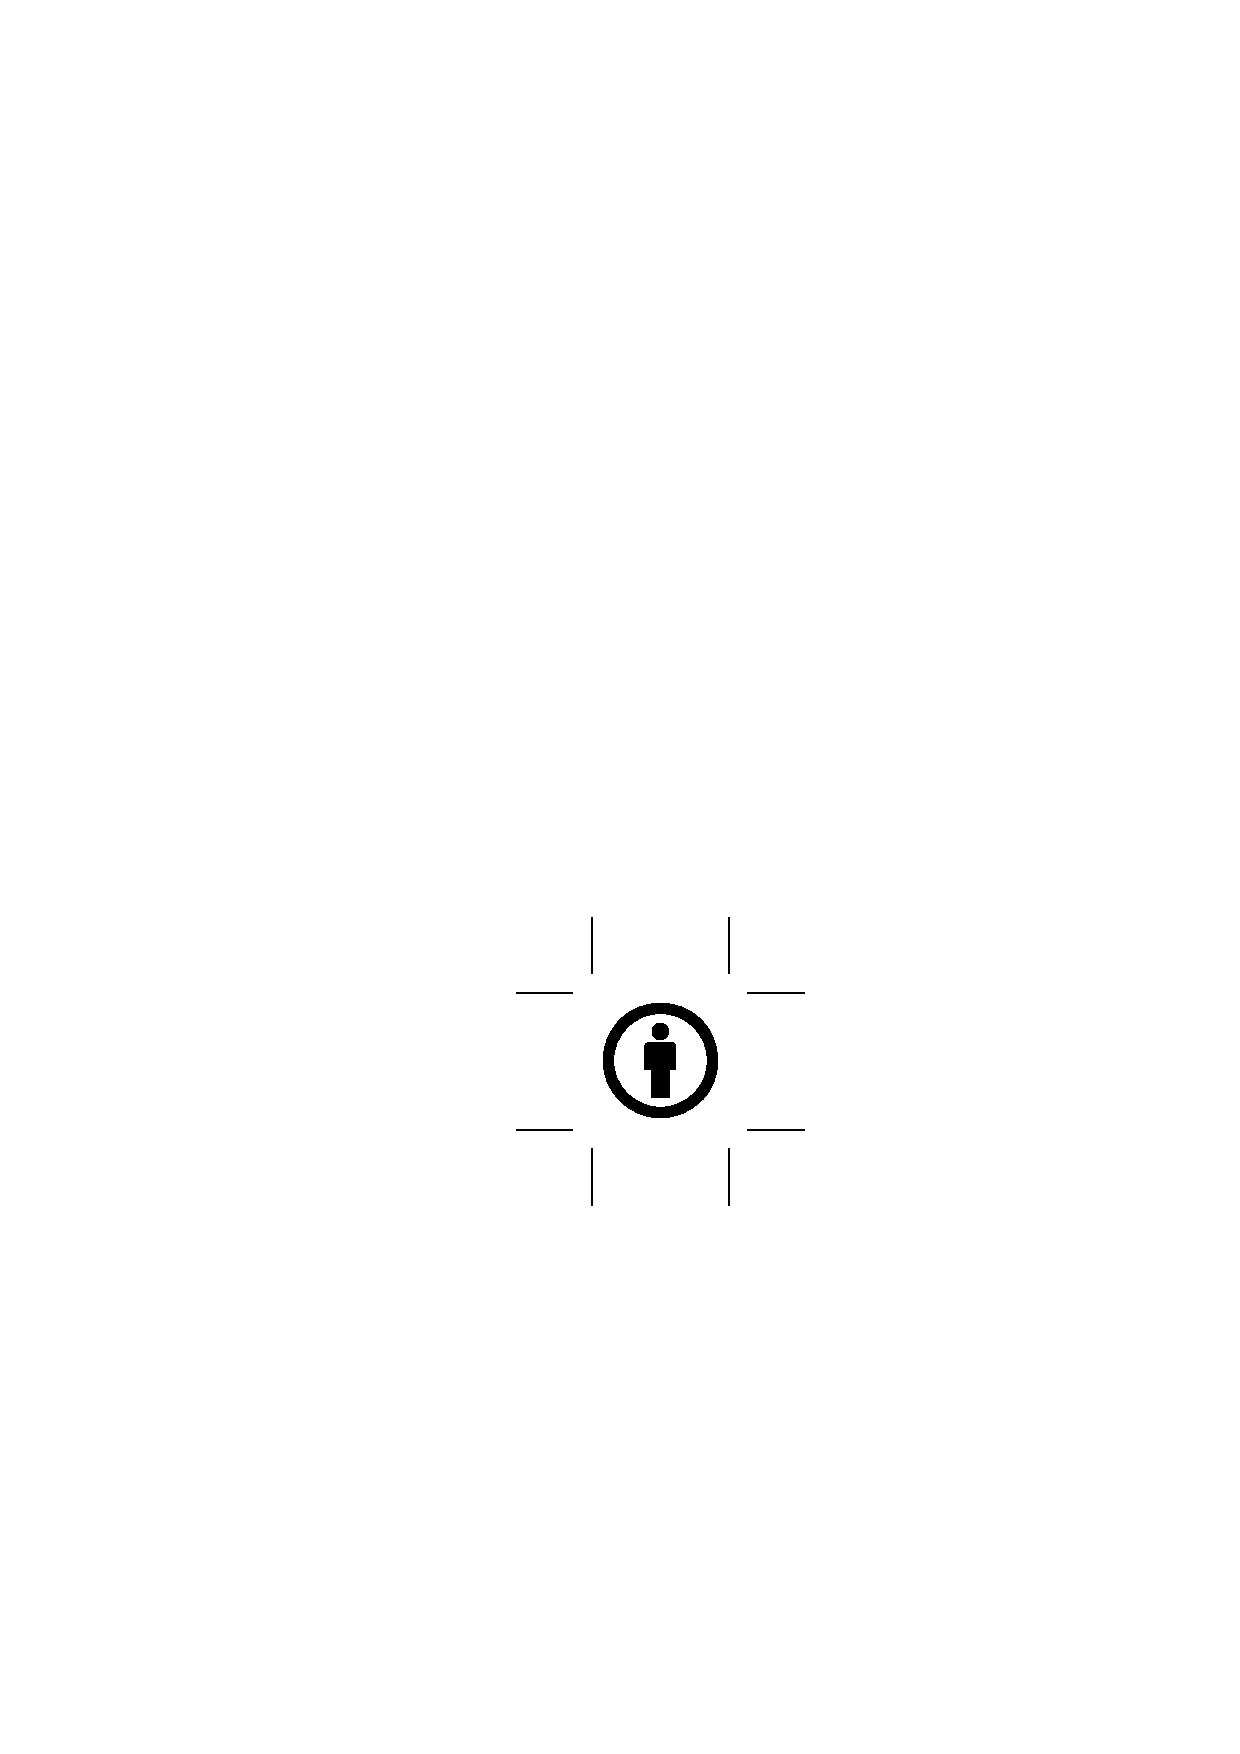
\includegraphics[height=4ex]{gfx/logos/creativecommons/by}

\smallskip

\noindent%
Veröffentlicht unter \emph{Namensnennung 4.0 International (CC BY 4.0)} \\
\url{https://creativecommons.org/licenses/by/4.0/deed.de}

\end{otherlanguage}

\smallskip

\noindent%
Licensed under \emph{Attribution 4.0 International (CC BY 4.0)} \\
\url{https://creativecommons.org/licenses/by/4.0/deed.en}

	\cleardoublepage% !TeX root = ../Thesis.tex

%*******************************************************
% Dedication
%*******************************************************
\thispagestyle{empty}
\phantomsection
\pdfbookmark[1]{Dedication}{Dedication}

\vspace*{3cm}

\begin{center}
    \emph{Ohana} means family. \\
    Family means nobody gets left behind, or forgotten. \\ \medskip
    --- Lilo \& Stitch
\end{center}

\medskip

\begin{center}
    Dedicated to the loving memory of Rudolf Miede. \\ \smallskip
    1939\,--\,2005
\end{center}

}{
	% !TeX root = ../Thesis.tex

%*******************************************************
% Titlepage
%*******************************************************
\pdfbookmark[1]{Cover}{cover}
\begin{titlepage}
    %\pdfbookmark[1]{\myTitle{}}{titlepage}
    % if you want the titlepage to be centered, uncomment and fine-tune the line below (KOMA classes environment)
    \begin{addmargin}[-1cm]{\iftoggle{adrianstyle}{-2cm}{-3cm}}
    \begin{center}
        \large

        
\includegraphics[width=6cm]{gfx/logos/tud_logo}
        
        \vfill

        \begingroup
            \color{CTtitle}\spacedallcaps{\myTitle{}} \\ \bigskip
        \endgroup

        \spacedlowsmallcaps{\myName{}}

        \vfill

        \medskip

        \myDegree{} \\ \medskip
        \myTime{}

        \bigskip

        \vfill

        \myDepartment{} \\
        \myFaculty{} \\[0.2cm]
        %\myUni{} \\
        
\includegraphics[width=5cm]{gfx/logos/seemoo_logo} \\

        %\vfill
    \end{center}
    \end{addmargin}
\end{titlepage}

	% !TeX root = ../Thesis.tex

\thispagestyle{empty}

\noindent\myTitle{} \\
\noindent\myTitleGerman{} \\
\noindent\myDegree{} \\
\noindent\myThesiscode{}

\bigskip

\noindent Submitted by \myName{} \\
\noindent Date of submission: \myTime{}

\bigskip

\noindent Advisor: \myProf{}

\noindent Supervisor: \mySupervisor{}


\hfill

\vfill

\noindent \myUni{} \\
\noindent \myFaculty{} \\
\noindent \myDepartment{} \\
	
}
%\cleardoublepage\include{FrontBackmatter/Foreword}
\cleardoublepage% !TeX root = ../Thesis.tex

%*******************************************************
% Abstract
%*******************************************************
%\renewcommand{\abstractname}{Abstract}
\pdfbookmark[1]{Abstract}{Abstract}
% \addcontentsline{toc}{chapter}{\tocEntry{Abstract}}
\begingroup
\let\clearpage\relax
\let\cleardoublepage\relax
\let\cleardoublepage\relax

\chapter*{Abstract}

Today, advanced machine learning is deployed nearly everywhere, often to great success. Yet, the field of hardware high-level synthesis has experienced notably little of this recent trend. 

Deploying artificial neural networks in the Placement stage of the synthesis flow shows great potential for improvement over traditional approaches. Using neural network based wirelength estimation can enable high-quality placements at reduced runtimes on some circuits. Increased research into this application of deep neural networks is likely to yield generally applicable solutions, innovating the design flows established in the field of hardware synthesis.

\vfill

\begin{otherlanguage}{ngerman}
\pdfbookmark[1]{Zusammenfassung}{Zusammenfassung}
\chapter*{Zusammenfassung}

Fortgeschrittene Techniken des Maschinellen Lernens werden heutzutage quasi überall eingesetzt, oft mit großem Erfolg. Das Gebiet der Hardwaresynthese wurde jedoch merklich wenig von diesem aktuellen Trend beeinflusst.

Künstliche neuronale Netze in der Platzierungsphase des Synthesevorgangs einzusetzen zeigt großes Potenzial für Verbesserungen gegenüber traditionellen Ansätzen. Der Einsatz einer Verdrahtungslängenabschätzung basierend auf neuronalen Netzen kann auf gewissen Schaltungen qualitativ hochwertige Platzierungen bei verminderter Laufzeit ermöglichen. Verstärkte Forschung an diesem Einsatz von tiefen neuronalen Netzen wird mit hoher Wahrscheinlichkeit weitreichend anwendbare Lösungen hervorbringen, was die etablierten Designprozesse im Gebiet der Hardwaresynthese weiter verbessern würde.

\end{otherlanguage}

\endgroup

\vfill

\cleardoublepage% !TeX root = ../Thesis.tex

%*******************************************************
% Acknowledgments
%*******************************************************
\pdfbookmark[1]{Acknowledgments}{acknowledgments}

%\begin{flushright}{\slshape    
%    We have seen that computer programming is an art, \\ 
%    because it applies accumulated knowledge to the world, \\ 
%    because it requires skill and ingenuity, and especially \\
%    because it produces objects of beauty.} \\ \medskip
%    --- \defcitealias{knuth:1974}{Donald E. Knuth}%\citetalias{knuth:1974} \citep{knuth:1974}
%\end{flushright}



\bigskip

\begingroup
\let\clearpage\relax
\let\cleardoublepage\relax
\let\cleardoublepage\relax
\chapter*{Acknowledgments}
{\slshape 
I would like to express my deepest gratitude to my parents and my family for supporting me in all the years of my studies and also while writing this thesis.

\bigskip

Special thanks for giving helpful advice while writing this thesis goes to Dr.-Ing. Florian Stock.

}

\endgroup

\cleardoublepage% !TeX root = ../Thesis.tex

%*******************************************************
% Table of Contents
%*******************************************************
\pagestyle{scrheadings}
%\phantomsection
\pdfbookmark[1]{\contentsname}{tableofcontents}
\setcounter{tocdepth}{2} % <-- 2 includes up to subsections in the ToC
\setcounter{secnumdepth}{3} % <-- 3 numbers up to subsubsections
\manualmark
\markboth{\spacedlowsmallcaps{\contentsname}}{\spacedlowsmallcaps{\contentsname}}
\tableofcontents
\automark[section]{chapter}
\renewcommand{\chaptermark}[1]{\markboth{\spacedlowsmallcaps{#1}}{\spacedlowsmallcaps{#1}}}
\renewcommand{\sectionmark}[1]{\markright{\textsc{\thesection}\enspace\spacedlowsmallcaps{#1}}}
%*******************************************************
% List of Figures and of the Tables
%*******************************************************
\clearpage
% \pagestyle{empty} % Uncomment this line if your lists should not have any headlines with section name and page number
\begingroup
    \let\clearpage\relax
    \let\cleardoublepage\relax
    %*******************************************************
    % List of Figures
    %*******************************************************
    %\phantomsection
    %\addcontentsline{toc}{chapter}{\listfigurename}
    \pdfbookmark[1]{\listfigurename}{lof}
    \listoffigures

    \vspace{8ex}

    %*******************************************************
    % List of Tables
    %*******************************************************
    %\phantomsection
    %\addcontentsline{toc}{chapter}{\listtablename}
    \pdfbookmark[1]{\listtablename}{lot}
    \listoftables

    \vspace{8ex}
    % \newpage

    %*******************************************************
    % List of Listings
    %*******************************************************
    %\phantomsection
    %\addcontentsline{toc}{chapter}{\lstlistlistingname}
%    \pdfbookmark[1]{\lstlistlistingname}{lol}
%    \lstlistoflistings

%    \vspace{8ex}

    %*******************************************************
    % Acronyms
    %*******************************************************
    %\phantomsection
    \pdfbookmark[1]{Acronyms}{acronyms}
    \printglossary[type=\acronymtype]

\endgroup
\iftoggle{phd}{
	\cleardoublepage% !TeX root = ../Thesis.tex

%*******************************************************
\chapterExtra{Previously Published Material}
%*******************************************************
\label{ch:PreviousPublications}

This thesis includes material of previously published conference papers and articles. Following the regulations of the \myFaculty at \myUni, I list below the affected parts that include verbatim and rephrased fragments from these publications.

\sloppy

\paragraph{\Cref*{ch:introduction}}
\begin{itemize}
    \item \cref{sec:first_section} revises Section\,1 of all papers \dots
\end{itemize}

\fussy

\label{ch:PreviousPublicationsEnd}

	\cleardoublepage% !TeX root = ../Thesis.tex

%*******************************************************
% Collaborations
%*******************************************************
\chapterExtra{Collaborations}

% From Daniel Steinmetzer's dissertation
Systematically investigating a technical research topic and engineering the required tools is a demanding and interdisciplinary process. Most achievements could never evolve without collaborations in which colleagues and international partners integrated their intellectual forces. When working in teams, accounting particular contributions and components of the resulting publications to individual collaborators becomes almost impossible. This situation also applies to several contents of this thesis, which arise from collaborations, thus, cover joint contributions. Many of these collaborations persisted even longer than the research projects and became a long-term strategic partnership.
In our previous publications, all authors contributed by discussing ideas and debating on results throughout the whole project duration. Each of them has particular strengths that sometimes appear invisible. For this reason, I explicitly state and acknowledge---where possible---the contributions of my collaborators in the following.   

}{}
%********************************************************************
% Mainmatter
%*******************************************************
\cleardoublepage
\pagestyle{scrheadings}
\pagenumbering{arabic}
%\setcounter{page}{90}
% use \cleardoublepage here to avoid problems with pdfbookmark
\cleardoublepage
\iftoggle{parts}{
	\ctparttext{The first chapter of this part gives an introduction and a motivation to this thesis, followed by a presentation of related work found in the area of physical layer security. In the third chapter, we present some definitions and background information to make it easier for the reader to quickly understand the subsequent parts of this thesis.}
	\part{Introduction}
}{}
% !TeX root = ../Thesis.tex

%************************************************
\chapter{Introduction}\label{ch:introduction}
%************************************************
\glsresetall % Resets all acronyms to not used

Start a chapter with text and not with a section header. Open the
\emph{classicthesis-config.tex} file to insert the title of your thesis, the
names of your supervisors and the hand-in date of your thesis.

\section{First Section}
\label{sec:first_section}

After a section there should always be text before the next section. The first
paragraph is always without indentation. Starting from the second paragraph,
there is an indentation.

Here is an equation without numbers for referencing:
\begin{align*}
\underbrace{\begin{pmatrix}\mathcal{B}_1\\\mathcal{B}_2\\\vdots\\\mathcal{B}_R\end{pmatrix}}_\mathcal{B} &= \underbrace{\begin{pmatrix}H_{1,1} & H_{1,2} & \hdots & H_{1,T}\\H_{2,1} & H_{2,2} & \hdots & H_{2,T}\\\vdots & \vdots & \ddots & \vdots\\H_{R,1} & H_{R,2} & \hdots & H_{R,T}\end{pmatrix}}_{H_{A\rightarrow B}}\cdot \underbrace{\begin{pmatrix}\mathcal{A}_1\\\mathcal{A}_2\\\vdots\\\mathcal{A}_T\end{pmatrix}}_\mathcal{A}
\end{align*}

Here is an equation that you can reference:
\begin{align}
\underbrace{\begin{pmatrix}\mathcal{B}_1\\\mathcal{B}_2\\\vdots\\\mathcal{B}_R\end{pmatrix}}_\mathcal{B} &= \underbrace{\begin{pmatrix}H_{1,1} & H_{1,2} & \hdots & H_{1,T}\\H_{2,1} & H_{2,2} & \hdots & H_{2,T}\\\vdots & \vdots & \ddots & \vdots\\H_{R,1} & H_{R,2} & \hdots & H_{R,T}\end{pmatrix}}_{H_{A\rightarrow B}}\cdot \underbrace{\begin{pmatrix}\mathcal{A}_1\\\mathcal{A}_2\\\vdots\\\mathcal{A}_T\end{pmatrix}}_\mathcal{A}\label{eqn:example}
\end{align}

\subsection{Referencing}

Take a look in the following list to reference sections, figures and equations:
\begin{itemize}
  \item \Cref{sec:first_section}
  \item \Cref{fig:wiretapchannel}
  \item \Cref{eqn:example}
\end{itemize}

\subsection{Acronyms}
For acronyms you should use the \emph{glossaries} package and put your acronyms
in the \emph{FrontBackmatter/acronyms.tex} file. The first acronym is always
written in it's long form, the following occurrences are abbreviated: first
occurrence \gls{SNR}, second occurrence \gls{SNR}, plural \glspl{SNR}.

\subsection{Examples on Figures}

\sloppy
When using figures, use vector graphics whenever possible. In
\cref{fig:wiretapchannel,fig:example} are some examples to
generate vector graphics directly from \LaTeX code. The second example is based
on the \emph{matlab2tikz} script for matlab. You find an example in the
\mbox{\emph{gfx/matlab/create\_example\_graph.m}} file. TikZ is used to generate
the graphics. As it takes some time and memory to recompile a graphic, pdflatex
caches generated figures when the \lstinline|--enable-write18| switch is set
when calling \lstinline|pdflatex|. Graphics are only recompiled when you
uncomment the \lstinline|\tikzset{external/remake next}| command. Figures should
always appear after the first reference in the text or at the top of the same
page as the reference, but never before the reference. Prefer placing figures on
separate pages. Try to always have figures and text on each page. Or place
enough figures to fill a page only with figures.

\begin{figure}
\centering
\begin{tikzpicture}[node distance=6mm]
\node[dspsquare,minimum height=3.2em, minimum width=5em,text height=1em, fill=white]
		(source) {Source};
\node[dspsquare,minimum height=3.2em, minimum width=5em,text height=1em, fill=white, right=of source]
		(encoder) {Encoder};
\node[dspsquare,minimum height=3.2em, minimum width=7em,text height=2em, fill=white, right=of encoder]
		(mainch) {Main Channel\\$Q_M$};
\node[dspnodefull, right=of mainch] (n1) {};
\node[dspsquare,minimum height=3.2em, minimum width=5em,text height=1em, fill=white, right=of n1]
		(decoder) {Decoder};
\node[coordinate,right=of decoder] (n2) {};
\node[dspsquare,minimum height=3.2em, minimum width=10em,text height=2em, fill=white, below=1cm of n1]
		(wiretapch) {Wiretap Channel\\$Q_W$};
\node[coordinate,below=of wiretapch] (n3) {};

\draw[dspconn] (source) -- node[midway,above] {$S^K$} (encoder);
\draw[dspconn] (encoder) -- node[midway,above] {$X^N$} (mainch);
\draw[dspconn] (mainch) -- node[midway,above] {$Y^N$} (decoder);
\draw[dspconn] (decoder) -- node[midway,above] {$S^K$} (n2);
\draw[dspconn] (n1) -- (wiretapch);
\draw[dspconn] (wiretapch) -- (n3) node[below] {$Z^N$};
\end{tikzpicture}
\caption[The wiretap channel]{The wiretap channel (source: \cite{1975:Wyner})}
\label{fig:wiretapchannel}
\end{figure}

\subsection{Examples on Tables}

You can find an example table in \cref{tab:disasters} using the \emph{tabular} environment. Note the use of horizontal lines from the \emph{booktabs} package (\lstinline|\toprule|, \lstinline|\midrule|, and \lstinline|\bottomrule|) and removed whitespace at both sides of the table (\lstinline|@{}|) as proposed by Markus Püschel.\footnote{\url{https://www.inf.ethz.ch/personal/markusp/teaching/guides/guide-tables.pdf}}

\begin{table}
\centering
\begin{tabular}{@{} lclr @{}} % @{} removes white spaces
	\toprule
	\tableheadline{Disaster} & \tableheadline{Year} & \tableheadline{Country} & \tableheadline{Area (km\textsuperscript{2})} \\
	\midrule
	Nepal earthquake & 2015 & Nepal & 3\,610 \\
	Cyclone Pam & 2015 & Vanuatu & 12\,190 \\
	Ludian earthquake & 2014 & China & 1\,487 \\
	Typhoon Haiyan & 2013 & Philippines & 71\,503 \\
	Christchurch earthquake & 2011 & New Zealand & 1\,426 \\
	East Africa drought & 2011 & East Africa & 2\,346\,466 \\
	Tropical storm Washi & 2011 & Philippines & 104\,530 \\
	Tohoku earthquake & 2011 & Japan & 83\,955 \\
	Haiti earthquake & 2010 & Haiti & 27\,750 \\
	Afghanistan blizzard & 2008 & Afghanistan & 652\,864 \\
	Sichuan earthquake & 2008 & China & 485\,000 \\
	Cyclone Nargis & 2008 & Myanmar & 676\,578 \\
	\bottomrule
\end{tabular}
\caption{Large-scale natural disasters in the last ten years}
\label{tab:disasters}
\end{table}

\section{Margin Notes}

Especially in the standard SEEMOO template with wide margins, you are
\marginpar{Here you can add text to the margin. For example, to
summarize the section next to it.} encouraged to insert text into the
margins. If you decide to do so, plan to have at least one margin note
per double page.

\section{Some Example Text}
\lipsum[3]

\begin{figure}
\centering
\setlength\figureheight{5cm}
\setlength\figurewidth{0.86\textwidth}
% uncomment the following line to recompile the figure when it changes otherwise a cached version is used
%\tikzset{external/remake next}
% This file was created by matlab2tikz v0.4.7 running on MATLAB 8.1.
% Copyright (c) 2008--2014, Nico Schlmer <nico.schloemer@gmail.com>
% All rights reserved.
% Minimal pgfplots version: 1.3
% 
% The latest updates can be retrieved from
%   http://www.mathworks.com/matlabcentral/fileexchange/22022-matlab2tikz
% where you can also make suggestions and rate matlab2tikz.
% 
\begin{tikzpicture}[%
font=\footnotesize
]

\begin{axis}[%
width=\figurewidth,
height=\figureheight,
scale only axis,
xmin=1,
xmax=100,
xlabel={x axis},
ymin=-1.5,
ymax=1.5,
ylabel={y axis},
legend style={draw=black,fill=white,legend cell align=left},
clip mode=individual,transpose legend,legend columns=2,legend style={at={(0,1)},anchor=north west,draw=black,fill=white,legend cell align=left}
]
\addplot [color=blue,solid]
  table[row sep=crcr]{1	0.309016994374947\\
2	0.587785252292473\\
3	0.809016994374947\\
4	0.951056516295154\\
5	1\\
6	0.951056516295154\\
7	0.809016994374947\\
8	0.587785252292473\\
9	0.309016994374948\\
10	1.22464679914735e-16\\
11	-0.309016994374947\\
12	-0.587785252292473\\
13	-0.809016994374947\\
14	-0.951056516295154\\
15	-1\\
16	-0.951056516295154\\
17	-0.809016994374948\\
18	-0.587785252292473\\
19	-0.309016994374948\\
20	-2.44929359829471e-16\\
21	0.309016994374947\\
22	0.587785252292472\\
23	0.809016994374947\\
24	0.951056516295154\\
25	1\\
26	0.951056516295154\\
27	0.809016994374948\\
28	0.587785252292473\\
29	0.309016994374948\\
30	3.67394039744206e-16\\
31	-0.309016994374947\\
32	-0.587785252292473\\
33	-0.809016994374947\\
34	-0.951056516295153\\
35	-1\\
36	-0.951056516295154\\
37	-0.809016994374948\\
38	-0.587785252292473\\
39	-0.309016994374948\\
40	-4.89858719658941e-16\\
41	0.309016994374945\\
42	0.587785252292473\\
43	0.809016994374947\\
44	0.951056516295153\\
45	1\\
46	0.951056516295154\\
47	0.809016994374947\\
48	0.587785252292474\\
49	0.30901699437495\\
50	6.12323399573677e-16\\
51	-0.309016994374945\\
52	-0.587785252292473\\
53	-0.809016994374948\\
54	-0.951056516295153\\
55	-1\\
56	-0.951056516295154\\
57	-0.809016994374949\\
58	-0.587785252292474\\
59	-0.30901699437495\\
60	-7.34788079488412e-16\\
61	0.309016994374948\\
62	0.587785252292472\\
63	0.809016994374948\\
64	0.951056516295153\\
65	1\\
66	0.951056516295154\\
67	0.809016994374949\\
68	0.587785252292474\\
69	0.309016994374947\\
70	8.57252759403147e-16\\
71	-0.309016994374948\\
72	-0.587785252292472\\
73	-0.809016994374946\\
74	-0.951056516295153\\
75	-1\\
76	-0.951056516295154\\
77	-0.809016994374947\\
78	-0.587785252292474\\
79	-0.309016994374947\\
80	-9.79717439317883e-16\\
81	0.309016994374945\\
82	0.587785252292469\\
83	0.809016994374948\\
84	0.951056516295153\\
85	1\\
86	0.951056516295154\\
87	0.809016994374949\\
88	0.587785252292477\\
89	0.309016994374947\\
90	1.10218211923262e-15\\
91	-0.309016994374945\\
92	-0.587785252292472\\
93	-0.809016994374946\\
94	-0.951056516295154\\
95	-1\\
96	-0.951056516295154\\
97	-0.809016994374949\\
98	-0.587785252292477\\
99	-0.309016994374947\\
100	-1.22464679914735e-15\\
};
\addlegendentry{sinus};

\end{axis}
\end{tikzpicture}%
\caption[Caption for list of figures]{Caption of figure}
\label{fig:example}
\end{figure}

\lipsum[6-10]

% !TeX root = ../Thesis.tex

%*****************************************
\chapter{Background}\label{ch:relatedwork}
%*****************************************
\glsresetall % Resets all acronyms to not used

We begin by giving an overview over the technologies and methods used and their domains.

\section{Hardware High-Level Synthesis}

Hardware high-hevel synthesis is the process of automatically translating an abstract high-level description of a circuits functionality into the actual specification of the hardware needed to realize it.

\subsection{The VTR Project and VPR}

The open-source \gls{VTR} project\cite{vtr8} provides a complete workflow of Verilog-to-Hardware translation for \gls{FPGA} architectures. It is targeted at research rather than production, and as such also includes various visualisation utilities and benchmarks of different sizes.

The workflow consists of three separate subprojects which can be run in series, but also independently: Odin II performing synthesis of a Verilog description to a \gls{BLIF} netlist, the external ABC project developed at UC Berkeley\cite{ABC-web} performing logic optimization, and the \gls{VPR} project generating and analysing the final layout.

As the name implies, \gls{VPR} performs placing and routing of the \gls{BLIF} netlist it receives as input, but also analyses the produced results with respect to timing and resource consumption.

\subsubsection{Netlists}

Netlists are a format of describing the logic of an abstract circuit, containing blocks and a list of nets.

Blocks are hardware primitives like \glspl{LUT}, \gls{I/O} pads, or basic logic functions, which usually are units of fixed dimensions connecting to the circuit via terminals acting either as signal sources or sinks. In a Netlist, blocks do not have coordinates yet, but are templates of the actual hardware components needed to perform the desired operation.

A Net is the abstraction of wires connecting specific terminals of the blocks referenced by the net. Each net has a single signal source, the output terminal of some block, which it connects to at least one input terminal of another (or possibly the same) block, its sinks.

In conjunction, these describe the full logical signal paths of a circuit, fully defining its logical behaviour.

\gls{BLIF} provides an open standard format for saving and interchanging logic-level circuit descriptions, enabling interaction of tools from different vendors or projects.\cite{blif-web} \gls{VPR} contains a packing tool to translate circuits in \gls{BLIF} format into Netlists, and therefore supports \gls{BLIF} circuits as input.

\subsubsection{Placement}

Placement is the process of assigning physical locations and orientations to the blocks of a Netlist. While on \glspl{FPGA} the orientation of a block is usually limited by the properties of the available resources at each location, the location itself for each block can be chosen rather freely. However, it is the main task of Placement to choose placements intelligently, so that resource consumption is minimized and performance of the resulting physical circuit is maximized.

As the blocks need to be connected physically according to the logical connections listen in the Netlist, placing connected blocks close to each other reduces both the consumption of limited wiring resources, and signal delays, which impose a hard limit on the possible clock frequency of sequential logic.

in \gls{VPR}, the search for an optimal placement is conducted via a classical simulated annealing algorithm. Possible moves are the swapping of a blocks position with an other free or occupied valid position. The acceptance criterium of a move is the overall reduction of estimated wiring costs, and moves increasing this cost are accepted only with a certain variable probability.

Over a run of the algorithm the temporary placement converges towards a weighted local minimum of summed up estimated wiring costs and critical path length. Due to the ability to accept worsening moves, the simulated annealing algorithm is able to escape bad local minima and to generally produce "good" results. However, as it is a heuristic, no guarantees about the quality of the solution are given.

The quality improvement over increased runtime (controlled linearly by setting the number of moves per temperature level) behaves approximately logarithmically, with a tenfold runtime only achieving 10\% improved quality.\cite{vtr8}

It is this property that warrants our assumption that the algorithm can be improved by introducing a substantial increase in runtime in return for substantially more accurate wiring cost estimates.

\subsubsection{Routing}

Once the blocks are placed, they still need to be connected physically. Not only is a straight connection from signal source to sink usually not possible for most nets as different wires need to be electrically isolated from each other and subsequently must not simply cross, but once there are several sinks in a net, finding the ideal connection structure (lowest accumulated wire length) also becomes a np-hard problem\cite{rsmt-complexity}.

While smart placement can already minimize the need for crossing wires, a certain amount usually remains unavoidable on large circuits. On static architectures like \gls{PCB} or Silicon, this is usually compensated by introducing multiple physical layers via which wires can evade. On \glspl{FPGA} however, wires have to be routed through a grid of connection fabric, where each edge consists of a number of parallel wires called channels, which can be freely connected with any adjacent channel at intersection points by configuring a programmable connection matrix.

These limits in available wiring space/resources causes local bottlenecks, which usually require some of the nets to be connected non-ideally in order to meet global constraints and minimize resource usage. The process of specifying the physical wiring of all nets under global and local constraints is called Routing.

\gls{VPR} uses a greedy heuristics known as "rip-up and re-route" to achieve Routing. This roughly means routing net after net locally optimally using only the currently remaining resources. Once it is not possible at all to route a net because there are no resources left that would connect all the terminals, the algorithm backtracks and unroutes certain nets, freeing their routing resources.\cite{vtr8}

First and foremost, \gls{VPR} minimizes the global number of parallel channels available at each grid edge. This is achieved by imposing a hard limit, trying to route the circuit, and increasing the limit if no valid routing was found. If the circuit was routed successfully, the limit is reduced, until by manner of binary partitioning the minimum channel count is found.

For the local routing of a single net, the Maze-Router\cite{Maze-Router} algorithm is used, again a greedy heuristics, which is however guaranteed to produce results within a certain margin of the optimal solution (a \gls{RSMT}), as it is at least as good as the corresponding \gls{RMST}.\cite{rmst-quality}

\subsection{Wirelength Estimation}

Estimating the wiring cost of a temporary placement is a central part of the \gls{VPR} Placer. The global wiring cost is computed as the sum of the wiring costs of each net.

Here, the wiring cost is defined as the absolute distance of wiring required for each net. As the effects different nets have on each other are not known before routing the circuit, the wiring distance for each net is computed in isolation assuming abundant resources so any two points in the routing grid can be directly and minimally connected. Together with a uniform grid this results in the Manhattan-distance as cost of the connection between two points.

However, computing the minimal rectilinear tree connecting the source of a net with all its sinks is a np-hard problem in the number of sinks called \gls{RSMT}.\cite{rsmt-complexity} Furthermore, the wiring cost computation is located at the innermost part of the simulated annealing algorithm used for Placement, which makes it highly runtime-critical.

Therefore, computing the \gls{RSMT} is impractical, and instead a very simple heuristic is used to estimate the wiring cost of individual nets.

\subsubsection{\gls{HPWL}}

\gls{VPR} uses a scaled variant of the \gls{HPWL} metric, which constitutes a very rough but efficient heuristics for approximating the total path length of the \gls{RSMT} of a net.

\gls{HPWL} is defined as half the perimeter of the axis-aligned minimal \gls{BB} of the terminals connected by the net. It is trivially exact for the case of one and two sinks, and provides a lower bound to the minimal wiring cost outside this restriction. 

With increasing sink count, however, this heuristics tends to underestimate the real cost. To combat this behaviour, \gls{VPR} weighs \gls{HPWL} with empirically determined factors relative to the terminal count of a net. While this invalidates the lower-bound property, it generally produces substantially better results than pure \gls{HPWL}.

The reason such a simple and possibly inaccurate estimator was chosen is its efficiency: if the \gls{BB} of a net is known, the \gls{HPWL} can be computed in constant time. As the \glspl{BB} of each affected net are updated whenever a block is moved, which is again highly efficient and does not add to the asymptotic complexity of the Placement algorithm (as moves are at the same level of the program loop as computing the wiring cost, and updating all affected \glspl{BB} is less complex than this).

\subsubsection{Other Common Heuristics}

\begin{figure}
	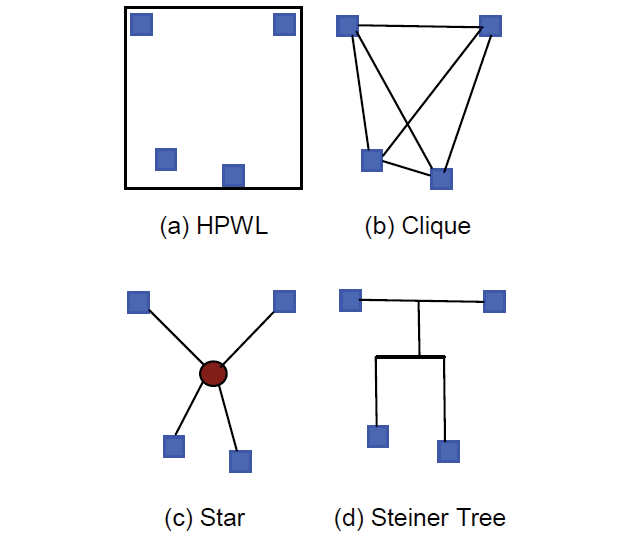
\includegraphics[width=\textwidth]{plots/wirelength-estimation-models.png}
	\caption{Popular wirelength estimation models. (source: \cite{star-plus-paper})}
	\label{fig:wirelength-estimation-models}
\end{figure}

Other popular approaches for in-placement wirelength estimation are the popular star+ model, the clique model, \glspl{RMST}, and \glspl{RSMT}.\cite{star-plus-paper}

While \gls{RSMT} provides the exact minimum possible wirelength, it is a np-hard problem and thus unsuited for in-placement estimation of iterative placers. \gls{RMST} is considerably faster than \gls{RSMT} and overestimates by 50\% at most\cite{rmst-quality}, it still exhibits a high complexity.

The clique model is in quality roughly equivalent as \gls{HPWL}\cite{star-plus-paper}, while being more complex and therefore inferior.

The star+ model on the other hand can be computed in constant time like \gls{HPWL}, but outperforms it measurably. This model estimates the wirelength of a net as the sum of distances from each terminal to the geometric centre of the net. It therefore processes more information than the simple \gls{HPWL} model, while still enabling a highly efficient computation.\cite{star-plus-paper}

\section{Neural Networks}

Neural Networks are universal function approximators based on a network of linear combinations followed by non-linear activation functions. They are a group of \gls{ML} algorithms learning their target function by initially making random predictions and improving through the observed error or effect of their predictions.

They usually consist of a layered structure of interconnected artificial neurons, essentially small units, which perform a linear combination of multiple inputs and produce a single output by adjusting that value through a non-linear activation function.

In their basic type, connections between neurons exist only from neurons in one layer to those in the directly adjacent higher layer. This creates a strict feed-forward semantic for prediction, and the weights of the linear combinations can be efficiently updated using a process called backpropagation.

\subsection{Regression}

The application of \glspl{NN} can be divided into Regression Problems and Classification Problems. 

Regression is the task of predicting the value of some variable or multiple variables, usually on a continuous domain, like future temperature prediction based on the weather data of the last few days, or estimating the age of a person depicted in an input image, but also predicting the pixel values of an image, essentially creating a new image.

Classification is the prediction of a discrete class label, e.g. classifying images whether they show cars or not. Classification can be realized as an extension of regression, by first predicting the probability of a certain class, and then introducing a threshold by which to decide if the input is considered part of that class or not.

\subsection{\glspl{CNN}}

\glspl{CNN} are a special class of \glspl{NN}, containing convolutional layers, which essentially implement learnable sliding-window filters over the input tensor. 

With their inherent ability to detect localized structures, \glspl{CNN} perform exceptionally well on image processing, essentially outperforming any other general-purpose image processing algorithm.\cite{dl-vs-cv}\cite{cv-vs-dl}

\subsection{\glspl{RNN}}

\glspl{RNN} contain a feedback loop, breaking the strict one-way forward pass semantic of usual \glspl{NN}. This causes \glspl{RNN} to contain state, enabling them to process sequences of related inputs, creating a single prediction for a sequence of input tensors.

\glspl{RNN} are usually used where the ordering of the input sequences contains relevant information, e.g. temporal sequences of sensor readings.

One important advantage of \glspl{RNN} is their inherent ability to process variable sized inputs without the need for padding or a size limit. While the input tensor dimensions are fixed, the sequence of inputs can have arbitrary length, with each additional tensor adjusting the internal state and thus the prediction.

One of the most popular types of \glspl{RNN} is the \gls{LSTM}\cite{lstm-paper}, a type of \gls{RNN} able to learn long-term dependencies, a task traditional \glspl{RNN} struggle with.\cite{lstm-web}

\subsection{Application in Wirelength Estimation}

In general, \glspl{NN} are able to approximate arbitrarily complex target functions\cite{universial-approx-web} within polynomial asymptotic complexity\cite{NN-complexity-web}. However, in praxis, even simple networks are often sufficient to obtain an estimator achieving very low prediction errors. Not only is the complexity of these estimators lower than their target function, but they also have low runtime in practice, making them faster even for small inputs.

Therefore, we believe \glspl{NN} could be suited as a wiring cost estimator by predicting the wiring cost of a the current placement of a net, receiving the coordinates of its terminals as inputs. 

They are expected to produce vastly more accurate estimations than the \gls{HPWL} metric, close to the real optimal wiring cost. Although they will also take substantially more computational effort than \gls{HPWL}, we expect the increased accuracy will help the simulated annealing placement algorithm to correctly judge the effects of its moves, which is an essential part of the algorithm. We hope that this will increase the resulting overall placement quality enough to be able to outperform the unchanged \gls{VPR} on the quality/runtime trade-off, being able to produce higher quality results at same actual runtime, by adjusting the moves per temperature level, at least on part of the runtime domain.

\subsubsection{Target Function}

Training a \gls{NN} using supervised learning requires training examples consisting of sample inputs and their expected prediction value, in our case terminal coordinates and the minimum wiring cost.

However, there are two competing candidates for the minimum wiring cost of a net placement: The \gls{RSMT}, specifying the minimum possible wiring cost, and the length of the wiring tree computed by the Maze-Router algorithm\cite{Maze-Router}, specifying the minimum wiring cost achievable by the \gls{VPR} Router, which might be higher than the \gls{RSMT} cost.

As our goal is to achieve optimal final results for the placed and routed circuit, we have to optimize the Placer to produce outputs optimal for the Router used, so the circuits can be routed efficiently. Therefore, we decided to use the cost computed using the Maze-Router algorithm, optimizing the placement for the routing algorithm present, not for a hypothetical ideal one.

\subsubsection{Related Work}

The deployment of \gls{ML} to \gls{FPGA} hardware synthesis is still rare\cite{routability-estimator}, and we identified only few publications closely related to our work. 

While there is one paper seemingly covering the same topic as our work, it is hidden behind a paywall, and the accessible abstract does not disclose much useful information.\cite{doi:10.1142/S0218213098000202}

In "Neural network based pre-placement wirelength estimation"\cite{pre-placement-estimation}, Liu et al. deploy \glspl{NN} to estimate wirelengths, however not on individual temporary net placements, but on whole circuits definitions.

Although not related to \glspl{NN}, the contents of the star+ paper incidentally exhibit strong parallels to our work. The authors also develop a in-placement wirelength estimator and evaluate it by implementing it into the \gls{VPR} Placer. The evaluation process deployed by Xu et al. is similar to our own in many aspects, but also contains important differences, as detailed in \ref{ch:evaluation}.

\iftoggle{parts}{
	\cleardoublepage
	\ctparttext{The contribution starts with a design chapter, where we mathematically describe the design of the physical layer security system, as well as the adaptive filter of the attacker. After the design follows the implementation on WARP nodes. Here we give an insight into the challenges of implementing the designed MIMO communication system. The last chapter concentrates on evaluating the performance of our proposed attack in simulation and practice.}
	\part{Contribution}
}{}
% !TeX root = ../Thesis.tex

%************************************************
\chapter{Design}\label{ch:design}
%************************************************
\glsresetall % Resets all acronyms to not used

Adding \glspl{NN} to \gls{VPR} consists of two parts: Designing and training the \glspl{NN}, and modifying the \gls{VPR} Placer to call them instead of the usual \gls{HPWL} routine.

\section{Problem Definition}

The problem to be solved with \glspl{NN}, that \gls{VPR} usually solves with \gls{HPWL}, is wirelength estimation.

The input is the temporary placement of a net, encoded as a list of 2D grid coordinates, with arbitrary length, but at least two entries. Each 2D coordinate is a pair of non-negative integers denoting the X and Y position of the terminal in the grid. 

The first element of the list specifies the position of a signal source, followed by the positions of all sinks connected to this source in the order in which they are stored in \gls{VPR}.

The output is the wiring cost for wiring this net in isolation using the Maze-Router. This is the minimum wire length achievable when greedily routing one terminal at a time in a fixed order.

\section{Neural Networks}

This thesis compares two different types of \glspl{NN} which are both suited to the problem at hand, namely \glspl{CNN} and \glspl{RNN}.

\subsection{\gls{CNN}}

Due to the discrete nature of possible placement positions on a \gls{FPGA}, every distinct pair of terminal coordinates represents a position on the equally spaced placement grid. 

As such, the grid itself can be represented by a binary-valued image (given a fixed grid size), where the pixels represent possible placement positions, and each value shows if the respective position contains a terminal of the current Net or if it is empty.

\subsubsection{Pros}

The main advantage of this approach is that every possible input can be converted to a tensor of fixed size, if a maximum grid size is specified, and each image represents this maximum grid. Therefore, samples converted in this way could already be processed by a single \gls{CNN} without further preprocessing, although quite inefficiently.

\subsubsection{Cons}

The main disadvantages are the memory-inefficient encoding, the loss of ordering information, and the limitation to a maximum grid size.

The encoding is an equivalent of a Bitmap, which is the most inefficient common image encoding in terms of memory requirement, as it contains no compression and has a fixed size given fixed dimensions.

In order to reduce the memory overhead of this approach, it is adapted to relative placement positions inside the bounding box of each Net, instead of absolute positions on the \gls{FPGA} grid. This reduces the memory requirement of each sample from the maximum placement grid size to the maximum bounding box size of all considered Net placements.

Furthermore, the ordering of the terminals inside a Net is lost. While the minimum possible wire length of a list of terminals is ordering invariant, the actual routing in \gls{VPR} is performed using the Maze-router, an ordering sensitive heuristic. Therefore, different internal orderings of the same list of terminal positions might produce routings of differing quality, and subsequently should be rated accordingly by the wire length estimation heuristic.

Our assumption at this point is that the influence of the ordering is small enough, that \glspl{CNN} are still able to perform better than \gls{HPWL} on the accuracy/runtime trade-off.

Finally, this approach is limited to a maximum grid, or rather Net placement bounding box, size. Any fixed size encoding can by design only represent problem instances up to a certain size. Therefore, any instance exceeding this limit can not be processed a \gls{CNN}. Furthermore, as the maximum size (number of grid positions) linearly influences the computational effort for each prediction, it is impractical to simply set the limit so high an excess becomes highly unlikely.

Therefore, to be able to process any valid input, a fallback estimator for problem instances exceeding the limit is required. While an ensemble of \glspl{CNN} with increasing input dimensions could combat the computational effort for prediction, it would require lots of resources for training, and still defines an upper limit that might be exceeded. Thus, a single \gls{CNN} able to process all commonly encountered Net placements on the \gls{VPR} benchmarks was chosen, and any placement exceeding this limit will fall back to \gls{HPWL}.

\subsection{\gls{RNN}}

In \gls{VPR}, the placement of the Terminals in a Net is represented by an ordered list of coordinates. The length of this list equals the number of terminals in the Net and is, in theory, unbounded. Due to the ordering sensitivity of the problem, and the variable-length input sequences, \glspl{RNN} are inherently suited to this problem.

This approach looks promising, as the computational structure of \glspl{RNN} mimics the process of sequentially adding a new terminal to the partial routing used in the Maze-router, which is the target function the \gls{NN} is trying to approximate.

The computational effort of this approach scales linearly with the number of terminals in a Net but is expected to be lower than the quasi-constant effort of \glspl{CNN}, as the number of terminals is generally lower than the number of distinct placement positions in the Nets \gls{BB}, by the maximum of which the effort of our CNN approach is scaled.

\section{Integration}

Each of the \glspl{NN}, wrapped in an interface, directly replaces the \gls{HPWL} heuristic used in the original \gls{VPR} implementation.

The interface pre-processes the input (the terminal coordinates of a net), executes the \gls{NN} inference, and post-processes the result to have the same unit as the cost computed by \gls{HPWL}.

However, parts of the \gls{HPWL} implementation, namely \gls{BB} computation and updating, are kept to map and normalize the input.

Thus, the actual cost computation part of the \gls{HPWL} implementation with constant runtime is replaced with \gls{NN} inference, which generally has substantially higher runtime. However, it is expected to also yield substantially more accurate wire length estimations, hopefully improving the placement quality enough to make up for the increased computational effort.



% !TeX root = ../Thesis.tex

%************************************************
\chapter{Implementation}\label{ch:implementation}
%************************************************
\glsresetall % Resets all acronyms to not used

\section{Training Data}



\subsection{Generation}

We generate training samples by logging real temporary placements of nets occurring during placing in \gls{VPR}.

\subsubsection{Data Source}

For this, we adapted the \gls{VPR} Placer to call our logging function whenever the \gls{HPWL} is computed for some net. We then placed the two benchmark circuits \textit{stereovision} and \textit{blob\_merge}, two of the largest \gls{VPR} benchmark circuits, saving the occurring net placements, which results in a huge number of samples from nets with a variety of terminal counts, with many samples for all small terminal counts, getting sparse towards higher values.

One full placement run, however, produces more samples than would be practical to process, so each run was terminated once the size of the plaintext logging file reached around \SI{100}{\mega\byte}.

\subsubsection{Target Value Computation}

Our choice of the target value for the training samples, the wiring cost for wiring a net in isolation using the Maze-Router, needs to be computed from the terminal coordinates of each net placement. While the Maze-Router is already implemented in the \gls{VPR} Router, it is not sufficiently isolated to be callable for a single placed net without significant overhead.

Therefore, we implemented the Maze-Router algorithm ourselves, working with the \gls{VPR} internal data structures holding the nets and their temporary placements.

\subsection{Format}

Before logging a sample, we call this algorithm to obtain the true wiring cost we are trying to learn to predict. We then log three lines of plaintext for each sample, containing all information necessary to reconstruct all relevant information about the temporary net placements:

\begin{itemize}
	\item \gls{BB} size: X and Y dimensions of the \gls{BB} of the terminal coordinates (this value is only included for convenience and could be computed from the corrdinates themselves)
	\item list of relative terminal coordinates: first the source terminal, then all sink terminals in the order they are stored in \gls{VPR}; coordinates relative to the lower-left corner of the \gls{BB}
	\item target value: the wiring cost computed using the Maze-Router
\end{itemize}

\subsection{Usage}

To use these samples for training a \gls{NN}, they need to be loaded again, and analysing the distribution of samples over terminal count revealed a need to partially balance these sample counts.

\subsubsection{Loading}

The loading of samples is done using a simple state machine looping over the lines of the text files.

\subsubsection{Balancing Terminal Counts}

TODO figures...

This imbalance causes our \glspl{RNN}\cite{TODO only lstms} to focus on correctly predicting the cost of net placements with a low terminal count, while neglecting samples with higher counts. While this imbalance is also present in "real" data, and one could argue that this behaviour was intentional to minimize overall error, placing nets with many terminals optimally is important, as these, although being rare, consume many more routing resources than simple nets.

To that end, we limit the samples per distinct terminal count to a fixed maximum. This limit is set to 4000, which was chosen empirically to be both low enough to sufficiently balance the data, and high enough not to waste samples unnecessarily.

\section{Neural Networks}

Although the \gls{VTR} project is implemented in C++, we implement and train our \glspl{NN} in Python for the convenience the various data processing libraries provide, and as our selected \gls{NN} framework, \gls{tf}, is primarily available for Python.

\subsection{\gls{tf} Framework}

\gls{tf} is a \gls{ML} framework specialized in Deep Learning.\cite{tensorflow2015-whitepaper} Since its 2.0 release in 2019, it implements the Keras interface\cite{chollet2015keras}, which simplifies model definition to stacking predefined layers types, only requiring to specify input and output tensor dimensions of the full network, as well as architectural parameters, such as neuron count, per layer.

\subsection{\gls{CNN}}



\subsubsection{Input Format}

For our \gls{CNN}, we have to map the input coordinates to an image. 

First, we subtract the lower-left corner of their \gls{BB}, which is known from the remaining part of the \gls{HPWL} implementation. This helps to reduce the maximum occurring coordinates.

We then prepare a black image (filled with 0-valued pixels) with a fixed size of 64x64px\cite{TODO}. Now, we set the value of the pixels at those coordinates to 1. This results in a binary-valued image, the lower-left corner of which directly maps to the \gls{BB} of the net placement, where all terminals which have to be connected are represented by pixels with a value of 1.

This scheme is only applicable for net placements with \glspl{BB} of no more than that size. However, this size was selected large enough so that all net placements occurring during the placement of the tested benchmarking circuits fit inside this limit. Indeed, the maximum \gls{BB} side length logged during training data generation is 54 units, therefore 64 units provides a certain upward margin for robustness. In the modified \gls{VPR} Placer, this limit is checked at runtime, and exceeding placements are handled by falling back to the original \gls{HPWL} computation.

By mapping coordinate values to pixel values, the sample inputs are automatically scaled to the range [0,1], making them appropriate for processing with \glspl{NN}.

The target value for each sample is the unscaled Maze-Router wiring cost, as this saves the effort of post-processing the output in the runtime-critical integration into \gls{VPR}.\cite{TODO}

\subsubsection{Structure}\label{ch:cnn-design}

To keep runtime small, the structure of our \glspl{CNN} is kept simple, with only few and small layers.

The general \gls{CNN} design, as illustrated in \ref{fig:cnn-structure-abstract}, consists of zero to two convolutional layers, followed by one to two dense layers. as the last layer, however, is always a dense layer with a single neuron, to achieve regression of one target variable, this leaves one to three custom layers. 

The special case of zero convolutional layers reduces the network to a plain artificial \gls{NN}, consisting only of dense layers. As these network variants, however, use the same encoding, and thus the same pre- and post-processing, they are treated the same as the remaining \glspl{CNN}. We not that this does, however, affect the integration of the \glspl{NN} into \gls{VPR}, as the entry point definition for the \gls{tf} API is dependent on the type of the input layer.

The neuron counts per dense layer are structured by two patterns, either with counts increasing to 16 neurons for the last hidden layer, or decreasing to 4.

The filter size of the convolutional layers can be 3x3 or 7x7, but is constant within all convolutional layers of a specific network.

\subsubsection{Training}

For this network, we use the standard training loop by calling the \textit{fit(...)} method of the \gls{tf} model, specifying training and validation data as well as number of epochs and batch size.

However, as using images to represent coordinates is an extremely inefficient encoding, and we have many samples (>1.000.000)\cite{TODO}, it is not possible with our available hardware to hold the full set of training data in memory. Therefore, we prepared the samples as \textit{tfrecord} files stored on disk, each holding 1.000 samples as advised by the documentation\cite{TODO}, and pass a generator to the fit method instead of the actual samples.

This generator, which is a slightly adapted version of the one used in a public project by \cite{TODO}, pre-loads several such files and shuffles the samples both externally and internally for a randomized ordering. This significantly reduces memory usage during training, but introduces an additional bottleneck, which causes the CPU utilization to drop.

The performance is logged using TensorBoard\cite{TODO}, and in the end the trained model is saved in the \gls{tf} SavedModel format\cite{TODO}, ready to be deployed to our adapted version of \gls{VPR}.

Early stopping, with a patience of 4, and checkpointing are deployed to automatically detect overfitting and save only the best weights evaluated during training of each model.

\subsection{\gls{RNN}}

\subsubsection{Input Format}

As the \gls{RNN} accepts sequences of variable length as input data, we encode the terminal positions as a ordered list of coordinate pairs.

To support efficient training we scale our training data. As the distribution of the terminals inside their \gls{BB} is approximately uniform (based on the properties of the simulated annealing placer), we normalize the coordinates to the range [0,1] by dividing by the maximum of their \glspl{BB}' X and Y dimensions. 

In the Maze-Router, all distances are computed using the Manhattan metric, and the result of the algorithm is a linear combination of distances. Therefore, linear scaling of the input values does not require recomputing the expected result, as the original result can simply be scaled using the same factor used when scaling the inputs.

As the scaling factor itself is not part of the input to the \gls{RNN}, it can only learn to predict the result of the scaled problem. Therefore, we need to post process the predicted output in our adapted \gls{VPR} implementation by rescaling it to the original magnitude using the inverse of the scaling factor of the inputs.

\subsubsection{Structure}\label{ch:rnn-design}

Similarly to the \gls{CNN} structure, our \glspl{RNN} are composed of \gls{LSTM} layers followed by dense layers (see \ref{fig:rnn-structure-abstract}). However, each \gls{RNN} has to contain at least one \gls{LSTM} layer, as the last \gls{LSTM} layer encodes the variable length sequences into fixed size tensors that can be processed by the following dense layers.

Thus, one to three \gls{LSTM} layers are followed by one or two dense layers, the last dense layer again being the fixed one-neuron output layer. Here, the neuron count is specified for both dense and \gls{LSTM} layers. The three patterns \textit{increasing}, \textit{decreasing}, and \textit{bloating} control the distribution of neurons over the layers, de- or increasing in steps of 4. \textit{Bloating} describes an increasing count within the \gls{LSTM} part of the network, and decreasing in the following dense layers.

\subsubsection{Training}

Although \glspl{RNN} generally support variable length input sequences, the implementation behind \gls{tf} imposes a limit on this: Input sequences within the same batch of samples are required to have uniform sequence length.

The standard \textit{fit(...)} method, however, only allows the user to specify the training data and batch size, but not to pass predefined batches.

As being able to predict the wiring cost with minimal preprocessing overhead is was the primary reason for choosing \glspl{RNN}, and a network trained only on samples padded to a common size would be unable to accurately predict on unpadded sequences, we implemented a custom training loop. This enables us to train on variably sized samples, by manually defining the batches.

Training with a batch size of 1, also called \textit{online learning}, would enable us to train on a sequence of samples with fully randomized ordering. However, this approach is generally known to not to converge to the same quality of or as stable results as minibatch learning, although being able to converge faster, i.e. on fewer samples. The runtime of the trained network, however, remains the same. As we are interested in getting as accurate predictions as possible for as little computation time as possible, and we have an abundance of training samples, we stick with minibatch learning.

For this, we model epochs by manually looping over the epoch count, and train on each batch separately using the \textit{fit()} method. We do not specify evaluation samples in the \textit{fit} calls, as the evaluation should only be done at the end of each epoch. To this end, we predict the wiring cost for each of the evaluation samples, and compute the metric score manually using the difference to the known true values.

The separation of training samples into batches is done only once in the beginning by sorting the samples by length, selecting consecutive ranges of samples with the same length as batches, and dropping the last non-full batch, if present.

To ensure a randomized order while training, we shuffle the batches both externally and internally each epoch, but we do not shuffle across batch borders for simplicity. We believe this to result in a sufficiently randomized ordering for efficient training.

Due to the custom training loop, the training of our \gls{RNN} model is not supported for supervision using TensorBoard. Therefore, we implemented simple logging and visualization to help in debugging and model selection.

Like our \gls{CNN}, the trained model is saved and can be deployed analogously. However, due to the custom training loop, early stopping and checkpointing are implemented explicitly, as the predefined callbacks can not be used in this scenario.

\section{Integration}

For integration of our \glspl{NN} into \gls{VPR}, which is implemented in C++, we modify the Placer in the central \textit{place.cpp} module. We implement an interface to our \glspl{NN} as an abstract class calling the \gls{NN} inference, implemented by a \gls{CNN} wrapper and a \gls{RNN} wrapper, performing model specific pre- and post-processing.

\subsection{\gls{tf} SavedModel}

The \glspl{NN} themselves are saved in the \gls{tf} SavedModel format, which faciliates portability across language bindings of the \gls{tf} framework. 
	
As the models are only used for inference, and will no longer be trained, we select not to include the optimizer in the saved model to save space.

\subsection{\gls{tf} C API}

The \gls{tf} C API provides language bindings for C++ as well as plain C. The executable code itself is loaded dynamically from the \textit{tensorflow.dll} dynamic link library.

However, it is not as well maintained as the Python library, and official releases are known often not to work. In our case, the precompiled dll was missing an entry point, so we needed to compile it from the source code. After fixing several incopatabilities and aquiring the necessary requirements, the compilation itself still took severel day, but succeeded eventually.

\subsection{Compile Time Integration into \gls{VPR} Placer}

As our modifications are located at the most performance-critical part of the \gls{VPR} Placer, we opted for compile time selection of operation mode to avoid introducing unnecessary control flow. 

We specified a compile time variable for four possible modes of operation: 

\begin{itemize}
	\item unchanged \gls{VPR}
	\item training data generation, writing all temporary net placements to a text file
	\item \gls{CNN} integration, replacing \gls{HPWL} with our \gls{CNN} interface for all nets with more than 3 terminals and placements not exceeding the hard limit
	\item \gls{RNN} integration, replacing \gls{HPWL} with our \gls{RNN} interface for all nets with more than 3 terminals
\end{itemize}

% !TeX root = ../Thesis.tex

%************************************************
\chapter{Evaluation}\label{ch:evaluation}
%************************************************
\glsresetall % Resets all acronyms to not used

To answer the main question of this thesis, whether the integration of \glspl{NN} into \gls{VPR} can improve its performance, we optimize and thoroughly evaluate our system.

\section{Evaluation Scenario}

First describing our method of evaluation as well as the specific settings used, we then evaluate the various \gls{NN} candidates against each other to determine the best network structure. Following this, the original \gls{VPR} Placer is evaluated and compared with our versions integrating \glspl{NN}.

\subsection{Selected Benchmarks}\label{ch:benchmarks}

For the final evaluation we select three circuits from the \gls{VPR} benchmark suite that we did not use in any prior part of this project, namely \textit{mcml.blif}, \textit{or1200.blif}, and \textit{diffeq2.blif}. The circuits are selected quasi-randomly, but ensuring that at least each one \textit{big} and one \textit{small} circuit is chosen.

In the same manner we also select an \textit{evaluation} set of one circuit (\textit{raygentop.blif}), which we will need for our chosen method of model selection, detailed in \ref{ch:model-selection}. This set is intentionally small to keep the computational effort of model selection manageable.

As the \gls{VPR} Placement algorithm is a pseudo-randomized heuristic not guarantee to yield reproducible results (when starting from a different state), each evaluation on each of this circuits will be averaged over 3 redundant placing attempts with different random seeds to ensure robust results.

\subsection{Runtime/Quality Trade-off}

Our metric of choice is runtime/quality trade-off, specifically discretely sampled routing quality (minimum channel width and critical path length) for certain approximate absolute placement run-times. These run-times, or sampling points, are selected per benchmark circuit relative to the runtime of the unchanged \gls{VPR} Placer (t\textsubscript{p}) as:

\begin{itemize}
	\item 1   * t\textsubscript{p}, or \textit{normal-mode}
	\item 10  * t\textsubscript{p}, or \textit{slow-mode}
	\item 50  * t\textsubscript{p}, or \textit{very-slow-mode}
	\item \cite{TODO} values might change when eval. is performed
\end{itemize}

The actual run-time, while not A-Priori \textit{predictable} for a certain configuration of the modified \gls{VPR} Placer, can easily be \textit{controlled} with the \textit{inner\_num} setting of \gls{VPR}.\cite{vtr8} 

Based on observations we state without formal proof that most of the computations of the \gls{VPR} Placer are performed inside each of these steps. Furthermore, while steps perform random actions and can have vastly differing run-time, within a certain \textit{temperature level} steps with different run-times are distributed randomly, and the number of steps per temperature is generally high. Therefore, changing this number of steps will not change the distribution of step run-times within a certain temperature-level, which means their average run-time remains approximately the same. Therefore, changes to the \textit{inner\_num} parameter, which is a linear factor for the actual number of steps performed, affect the total runtime of the modified \gls{VPR} Placer approximately linearly.

By placing a benchmark circuit using a fixed setting for \textit{inner\_num}, we acquire the runtime at this setting. As early experiments showed that the runtime of the \gls{VPR} Placer using \glspl{NN} is one to two orders of magnitude slower than using \gls{HPWL}, this value is set to $0.01*num_blocks^(4/3)$, which equals one hundredth of the default value of the \gls{VPR} Placer. Therefore, this first check is estimated to take approximately as much time as the unchanged \gls{VPR} in \textit{normal-mode}.

Now, \textit{inner\_num} can be scaled appropriately to gain quality scores at each sampling point.

Evaluating the performance of a certain \gls{NN} during model selection consists of the following steps:

\begin{itemize}
	\item integration into \gls{VPR}
	\item determining the runtime over \textit{inner\_num}
	\item setting \textit{inner\_num} appropriately for \textit{slow-mode}
	\item placing the evaluation circuit three times
	\item routing each placement and logging average quality 
\end{itemize}

The final evaluation of the best \gls{CNN} and \gls{RNN} against unchanged \gls{VPR} is performed as follows:

\begin{itemize}
	\item integration into \gls{VPR}
	\item determining the runtime over \textit{inner\_num}
	\item setting \textit{inner\_num} appropriately for \textit{normal-mode}
	\item placing the test circuits three times
	\item routing each placement and logging average quality per circuit
	\item repeating for \textit{slow-mode} and \textit{very-slow-mode}
\end{itemize}

The thus computed quality/runtime trade-off is then compared with that of the unchanged \gls{VPR} Placer.

As the \gls{VPR} Router primarily optimizes the \textit{channel width}, or maximum number of parallel routing channels used by the routing, by determining the minimum routable value via binary search, we select \textit{channel width} as the primary evaluation metric. In the final evaluation we will, however, also compare critical path lengths, as this, as \gls{VPR}'s secondary optimization target, defines the maximum operateable frequency of the circuit, directly influencing its computational capabilities.

\section{Model Selection}\label{ch:model-selection}

Although \glspl{NN} automatically tune their parameters to fit the target function, the structure and properties of the network itself has to be specified explicitly. While recent works try to automate even this, it is usually still necessary to manually design networks to achieve good results.

During model selection, \glspl{CNN} and \glspl{RNN} are evaluated independently from each other and using the same methodology. This yields a best \gls{CNN} and a best \gls{RNN}, which will both again be integrated into \gls{VPR} and evaluated against the unchanged Placer.  

\subsection{Empirical Model Search}

Typically, a first working design is found empirically through experimentation, based largely on best practices, related works, and intuition.\cite{TODO} In our case, the strict requirements on the runtime of the networks restricted the search space considerably, and the model candidates described in \ref{ch:cnn-design} and \ref{ch:rnn-design} represent the obvious choices for small and simple networks.

From these candidates, the best one is selected by evaluating each independently on evaluation data different from the training and the final test data, and comparing the results.

\subsection{\gls{HPO}}

As these groups of candidates are generated from discrete parameters, e.g. dense layer count, this model selection approach constitutes a grid search over these hyperparameters.

\cite{TODO} results of grid search

By evaluating the \gls{NN} candidates on the evaluation set at the \textit{slow-mode} sampling point we determine their relative performance. A visualization of the results in \ref{fig:eval-hyperopt-surface} clearly shows a correlation between network complexity and routing quality: Smaller networks produce better results, with the exception of \glspl{CNN} without convolutional layers. These models, using less time for a prediction, allow for a higher number of moves per temperature step, although producing less accurate predictions than their more complex counterparts. The properties of convolutional layers, while computationally being rather expensive (at least compared to the "tiny" dense layers), seem to be beneficial to accurately predict the wiring cost. As the \gls{LSTM} layers of the \glspl{RNN} are required to encode the input data for the following dense layers, their suitedness to the problem can not be measured that easily.

The exact results are presented in \ref{table:rnn-hyperopt-results} and \ref{table:cnn-hyperopt-results}. We thus select \textit{TODO} and \textit{TODO} as the best \gls{CNN} and \gls{RNN} models, respectively.

By comparing the performance to that of the unchanged \gls{VPR} Placer we can, however, also see, that none of the \glspl{NN} is able to beat \gls{HPWL} in \textit{slow-mode} (see \ref{fig:eval-hyperopt-surface-reference}).

\section{Results}

With a single network per type the modified \gls{VPR} Placer can now be evaluated against the unchanged version (reference system).

First, we present the performance of the reference system on our selected benchmarking test set. We then proceed by performing the same evaluation for our modified versions of the \gls{VPR} Placer, using \glspl{CNN} and\glspl{RNN}, respectively. A comprehensive comparison will answer the main question of this thesis, whether \gls{VPR} can be improved by replacing the crude \gls{HPWL} metric with more accurate, but also more expensive \glspl{NN}. Finally, we discuss our results and try to explain the observed behaviour.

\subsection{Reference System (Unchanged \gls{VPR})}

\subsection{\gls{CNN} Integration}

\subsection{\gls{RNN} Integration}

\subsection{Comparison}

\subsection{Justification}

covers discussion chapter?

\iftoggle{parts}{
	\cleardoublepage
	\ctparttext{After the evaluation, we further discuss the results and give an outlook. In addition, we finish this work with conclusions.}
	\part{Discussion and Conclusions}
}{}
% !TeX root = ../Thesis.tex

%************************************************
\chapter{Discussion}\label{ch:Discussion} % $\mathbb{ZNR}$
%************************************************
\glsresetall % Resets all acronyms to not used

\lipsum[6]

% !TeX root = ../Thesis.tex

%************************************************
\chapter{Conclusions}\label{ch:Conclusions}
%************************************************
\glsresetall % Resets all acronyms to not used

In this thesis we implemented in-placement wirelength estimation using \glspl{NN} by modifying the open \gls{VPR} project. We also investigated the feasibility of this approach by evaluating our modified versions of the \gls{VPR} Placer against the unchanged reference system. We detailed our approach and design choices, as well as our concrete implementation.

The evaluation showed that... TODO

We finally discussed our results, mentioning possible problems and outlining future work.

% ********************************************************************
% Backmatter
%*******************************************************
\iftoggle{parts}{}{
	\addtocontents{toc}{\protect\vspace{\beforebibskip}} % add space between main chapters and appendix if we do not use parts
}
\appendix
%\renewcommand{\thechapter}{\alph{chapter}}
\cleardoublepage
\iftoggle{parts}{
	\part{Appendix}
}{}
%% !TeX root = ../Thesis.tex

%********************************************************************
% Some Proof (Appendix)
%*******************************************************
% If problems with the headers: get headings in appendix etc. right
%\markboth{\spacedlowsmallcaps{Appendix}}{\spacedlowsmallcaps{Appendix}}
\chapter{Some Proof}\label{ch:SomeProof}
\glsresetall % Resets all acronyms to not used

\lipsum[8]

%********************************************************************
% Other Stuff in the Back
%*******************************************************
% Ugly hack: all remaining chapter bookmarks should be on the top level (not under Appendix)
\makeatletter
\renewcommand{\toclevel@chapter}{-1}
\renewcommand{\toclevel@section}{0}
\renewcommand{\toclevel@subsection}{1}
\renewcommand{\toclevel@subsubsection}{2}
\renewcommand{\toclevel@paragraph}{3}
\renewcommand{\toclevel@subparagraph}{4}
\makeatother

\cleardoublepage% !TeX root = ../Thesis.tex

%********************************************************************
% Bibliography
%*******************************************************
% work-around to have small caps also here in the headline
% https://tex.stackexchange.com/questions/188126/wrong-header-in-bibliography-classicthesis
% Thanks to Enrico Gregorio
\defbibheading{bibintoc}[\bibname]{%
  \phantomsection
  \manualmark
  \markboth{\spacedlowsmallcaps{#1}}{\spacedlowsmallcaps{#1}}%
  \addtocontents{toc}{\protect\vspace{\beforebibskip}}%
  \addcontentsline{toc}{chapter}{\tocEntry{#1}}%
  \chapter*{#1}%
}
\printbibliography[heading=bibintoc]

% Old version, will be removed later
% work-around to have small caps also here in the headline
%\manualmark
%\markboth{\spacedlowsmallcaps{\bibname}}{\spacedlowsmallcaps{\bibname}} % work-around to have small caps also
%\phantomsection
%\refstepcounter{dummy}
%\addtocontents{toc}{\protect\vspace{\beforebibskip}} % to have the bib a bit from the rest in the toc
%\addcontentsline{toc}{chapter}{\tocEntry{\bibname}}
%\label{app:bibliography}
%\printbibliography

\iftoggle{phd}{
	\cleardoublepage% !TeX root = ../Thesis.tex

%*******************************************************
% Publications
%*******************************************************
\chapterExtra{Author's Publications}

This might come in handy for PhD theses: some ideas and figures have appeared previously in the following publications:

\begin{refsection}[ownpubs]
    \small
    \nocite{*} % is local to to the enclosing refsection
    \printbibliography[heading=none]
\end{refsection}

\emph{Attention}: This requires a separate run of \texttt{bibtex} for your \texttt{refsection}, \eg, \texttt{ClassicThesis1-blx} for this file. You might also use \texttt{biber} as the backend for \texttt{biblatex}. See also \url{http://tex.stackexchange.com/questions/128196/problem-with-refsection}.

	\cleardoublepage% !TeX root = ../Thesis.tex

%************************************************
\chapterExtra{Curriculum Vit\ae}\label{ch:CurriculumVitae}
%************************************************

\begin{cv}{}

\renewcommand*{\cvlistheadingfont}{\spacedlowsmallcaps} % same as sections
\renewcommand*{\cvlabelfont}{\itshape}
\setlength\cvlabelwidth{60pt}

\begin{cvlist}{{Personal Information}}
    \item[Name] \myName
    \item[Date of Birth] \myBirthDate
    \item[Place of Birth] \myBirthPlace
    \item[Nationality] \myNationality
\end{cvlist}


\begin{cvlist}{{Education}}

\item[since 2018] \textbf{Doctoral Candidate} \\
Computer Science, Technische Universiät Darmstadt, Darmstadt, Germany

\item[2016--2018] \textbf{Master of Science} \\
Computer Science, Technische Universität Darmstadt, Darmstadt, Germany

\item[2013--2016] \textbf{Bachelor of Science} \\
Computer Science, Technische Universität Darmstadt, Darmstadt, Germany

\end{cvlist}


\begin{cvlist}{{Work Experience}}

\item[since 2012] \textbf{Research Associate} \\
Secure Mobile Networking Lab, Technische Universität Darmstadt, Darmstadt, Germany.

\end{cvlist}


\begin{cvlist}{{Awards}}

\item[Publication] \textbf{Best Community Paper Award at ACM MobiCom '18} \\
Paper: \enquote{One Billion Apples’ Secret Sauce: Recipe for the Apple Wireless Direct Link Ad hoc Protocol}.

\end{cvlist}        


\begin{cvlist}{{Supervised Student Theses}}

\item[B.\,Sc. Thesis] \textbf{Another Student}, \enquote{A Very Cool Topic}, 2018.

\item[M.\,Sc. Thesis] \textbf{Milan Schmittner}, \enquote{Scalable and Secure Multicast Routing for Mobile Ad-hoc Networks}, 2014.

\end{cvlist}


% \begin{cvlist}{{Miscellaneous}}

% \item[Teaching] Organization of the integrated course \enquote{Network Security}.

% \end{cvlist}


\date{\myLocation{}, \myTime{}}

\end{cv}

	\cleardoublepage%!TEX root = ../Thesis.tex

\begin{otherlanguage}{ngerman}

%*******************************************************
\chapterExtra{Erklärung zur Dissertationsschrift}
%*******************************************************

% Promotionsordnung und mehr des FB 20
% https://www.informatik.tu-darmstadt.de/forschung_fb20/wissenschaftliche_karriere/promotion/index.de.jsp

\begin{flushright}
    \emph{\small gemäß §\,9 der Allgemeinen Bestimmungen der Promotionsordnung der \\
    \myUni{} vom \formatdate{12}{1}{1990} (ABI. 1990, S.\,658) \\
    in der Fassung der 8.\,Novelle vom \formatdate{1}{3}{2018}}
\end{flushright}
Hiermit versichere ich, \myName{}, die vorliegende Dissertationsschrift ohne Hilfe Dritter und nur mit den angegebenen Quellen und Hilfsmitteln angefertigt zu haben. Alle Stellen, die Quellen entnommen wurden, sind als solche kenntlich gemacht worden. Eigenzitate aus vorausgehenden wissenschaftlichen Veröffentlichungen werden in Anlehnung an die Hinweise des Promotionsausschusses \myFacultyDE{} zum Thema \textquote{Eigenzitate in wissenschaftlichen Arbeiten} (EZ-2014/10) in Kapitel \textquote{\emph{Previously Published Material}} auf \cpagerefrange*{ch:PreviousPublications}{ch:PreviousPublicationsEnd} gelistet. Diese Arbeit hat in gleicher oder ähnlicher Form noch keiner Prüfungsbehörde vorgelegen. In der abgegebenen Dissertationsschrift stimmen die schriftliche und die elektronische Fassung überein.

\bigskip

\noindent\textit{\myLocation{}, \myTime{}}

\begin{flushright}
    \begin{tabular}{m{5cm}}
        \\ \hline
        \centering\myName{} \\
    \end{tabular}
\end{flushright}

\end{otherlanguage}

}{
	\cleardoublepage% !TeX root = ../Thesis.tex

%*******************************************************
% Declaration
%*******************************************************

% Text aus: https://www.intern.tu-darmstadt.de/media/dezernat_ii/referat_iig/formulare_vorlagen/pm_1/erklaerungen/Erklaerung_zur_Abschlussarbeit_Vorlage.docx
% Stand: 3. Juni 2019

\begingroup

\begin{otherlanguage}{ngerman}
\chapterExtra{Erklärung zur Abschlussarbeit}
\begin{flushright}
	\emph{gemäß §\,22 Abs.\,7 APB TU Darmstadt}
\end{flushright}

Hiermit versichere ich, \myName{}, die vorliegende \myDegree{} gemäß § 22 Abs. 7 APB der TU Darmstadt ohne Hilfe Dritter und nur mit den angegebenen Quellen und Hilfsmitteln angefertigt zu haben. Alle Stellen, die Quellen entnommen wurden, sind als solche kenntlich gemacht worden. Diese Arbeit hat in gleicher oder ähnlicher Form noch keiner Prüfungsbehörde vorgelegen. 

Mir ist bekannt, dass im Falle eines Plagiats (§38 Abs.2 APB) ein Täuschungsversuch vorliegt, der dazu führt, dass die Arbeit mit 5,0 bewertet und damit ein Prüfungsversuch verbraucht wird. Abschlussarbeiten dürfen nur einmal wiederholt werden.

\end{otherlanguage}

\vfill

\let\cleardoublepage\relax
\chapter*{Thesis Statement}
\begin{flushright}
	\emph{pursuant to §\,22 paragraph 7 of APB TU Darmstadt}
\end{flushright}

I herewith formally declare that I, \myName{}, have written the submitted thesis independently pursuant to § 22 paragraph 7 of APB TU Darmstadt. I did not use any outside support except for the quoted literature and other sources mentioned in the paper. I clearly marked and separately listed all of the literature and all of the other sources which I employed when producing this academic work, either literally or in content. This thesis has not been handed in or published before in the same or similar form.

I am aware, that in case of an attempt at deception based on plagiarism (§38 Abs. 2 APB), the thesis would be graded with 5,0 and counted as one failed examination attempt. The thesis may only be repeated once.

\vfill

\noindent\textit{\myLocation{}, \myTime{}}

\begin{flushright}
    \begin{tabular}{m{5cm}}
        \\ \hline
        \centering\myName{} \\
    \end{tabular}
\end{flushright}

\endgroup

}
%\cleardoublepage% !TeX root = ../Thesis.tex

\pagestyle{empty}

\hfill

\vfill


\pdfbookmark[0]{Colophon}{colophon}
\section*{Colophon}
This document was typeset using the typographical look-and-feel \texttt{classicthesis} developed by Andr\'e Miede and Ivo Pletikosić.
The style was inspired by Robert Bringhurst's seminal book on typography ``\emph{The Elements of Typographic Style}''.
\texttt{classicthesis} is available for both \LaTeX\ and \mLyX:
\begin{center}
\url{https://bitbucket.org/amiede/classicthesis/}
\end{center}
Happy users of \texttt{classicthesis} usually send a real postcard to the author, a collection of postcards received so far is featured here:
\begin{center}
\url{http://postcards.miede.de/}
\end{center}
Thank you very much for your feedback and contribution.

\bigskip

\noindent\finalVersionString

%Hermann Zapf's \emph{Palatino} and \emph{Euler} type faces (Type~1 PostScript fonts \emph{URW
%Palladio L} and \emph{FPL}) are used. The ``typewriter'' text is typeset in \emph{Bera Mono},
%originally developed by Bitstream, Inc. as ``Bitstream Vera''. (Type~1 PostScript fonts were made
%available by Malte Rosenau and
%Ulrich Dirr.)

%\paragraph{note:} The custom size of the textblock was calculated
%using the directions given by Mr. Bringhurst (pages 26--29 and
%175/176). 10~pt Palatino needs  133.21~pt for the string
%``abcdefghijklmnopqrstuvwxyz''. This yields a good line length between
%24--26~pc (288--312~pt). Using a ``\emph{double square textblock}''
%with a 1:2 ratio this results in a textblock of 312:624~pt (which
%includes the headline in this design). A good alternative would be the
%``\emph{golden section textblock}'' with a ratio of 1:1.62, here
%312:505.44~pt. For comparison, \texttt{DIV9} of the \texttt{typearea}
%package results in a line length of 389~pt (32.4~pc), which is by far
%too long. However, this information will only be of interest for
%hardcore pseudo-typographers like me.%
%
%To make your own calculations, use the following commands and look up
%the corresponding lengths in the book:
%\begin{verbatim}
%    \settowidth{\abcd}{abcdefghijklmnopqrstuvwxyz}
%    \the\abcd\ % prints the value of the length
%\end{verbatim}
%Please see the file \texttt{classicthesis.sty} for some precalculated
%values for Palatino and Minion.
%
%    \settowidth{\abcd}{abcdefghijklmnopqrstuvwxyz}
%    \the\abcd\ % prints the value of the length

% ********************************************************************
% Game Over: Restore, Restart, or Quit?
%*******************************************************
\end{document}
% ********************************************************************
